%-----------------------------------------------------------------------------%
% \addcontentsline{toc}{chapter}{LAMPIRAN 1}
% %\chapter*{Lampiran 1}
% \newappendix{Lampiran 1. Sertifikat HKI Aplikasi Mapping}
% \begin{figure}[H]
%   \centering
%   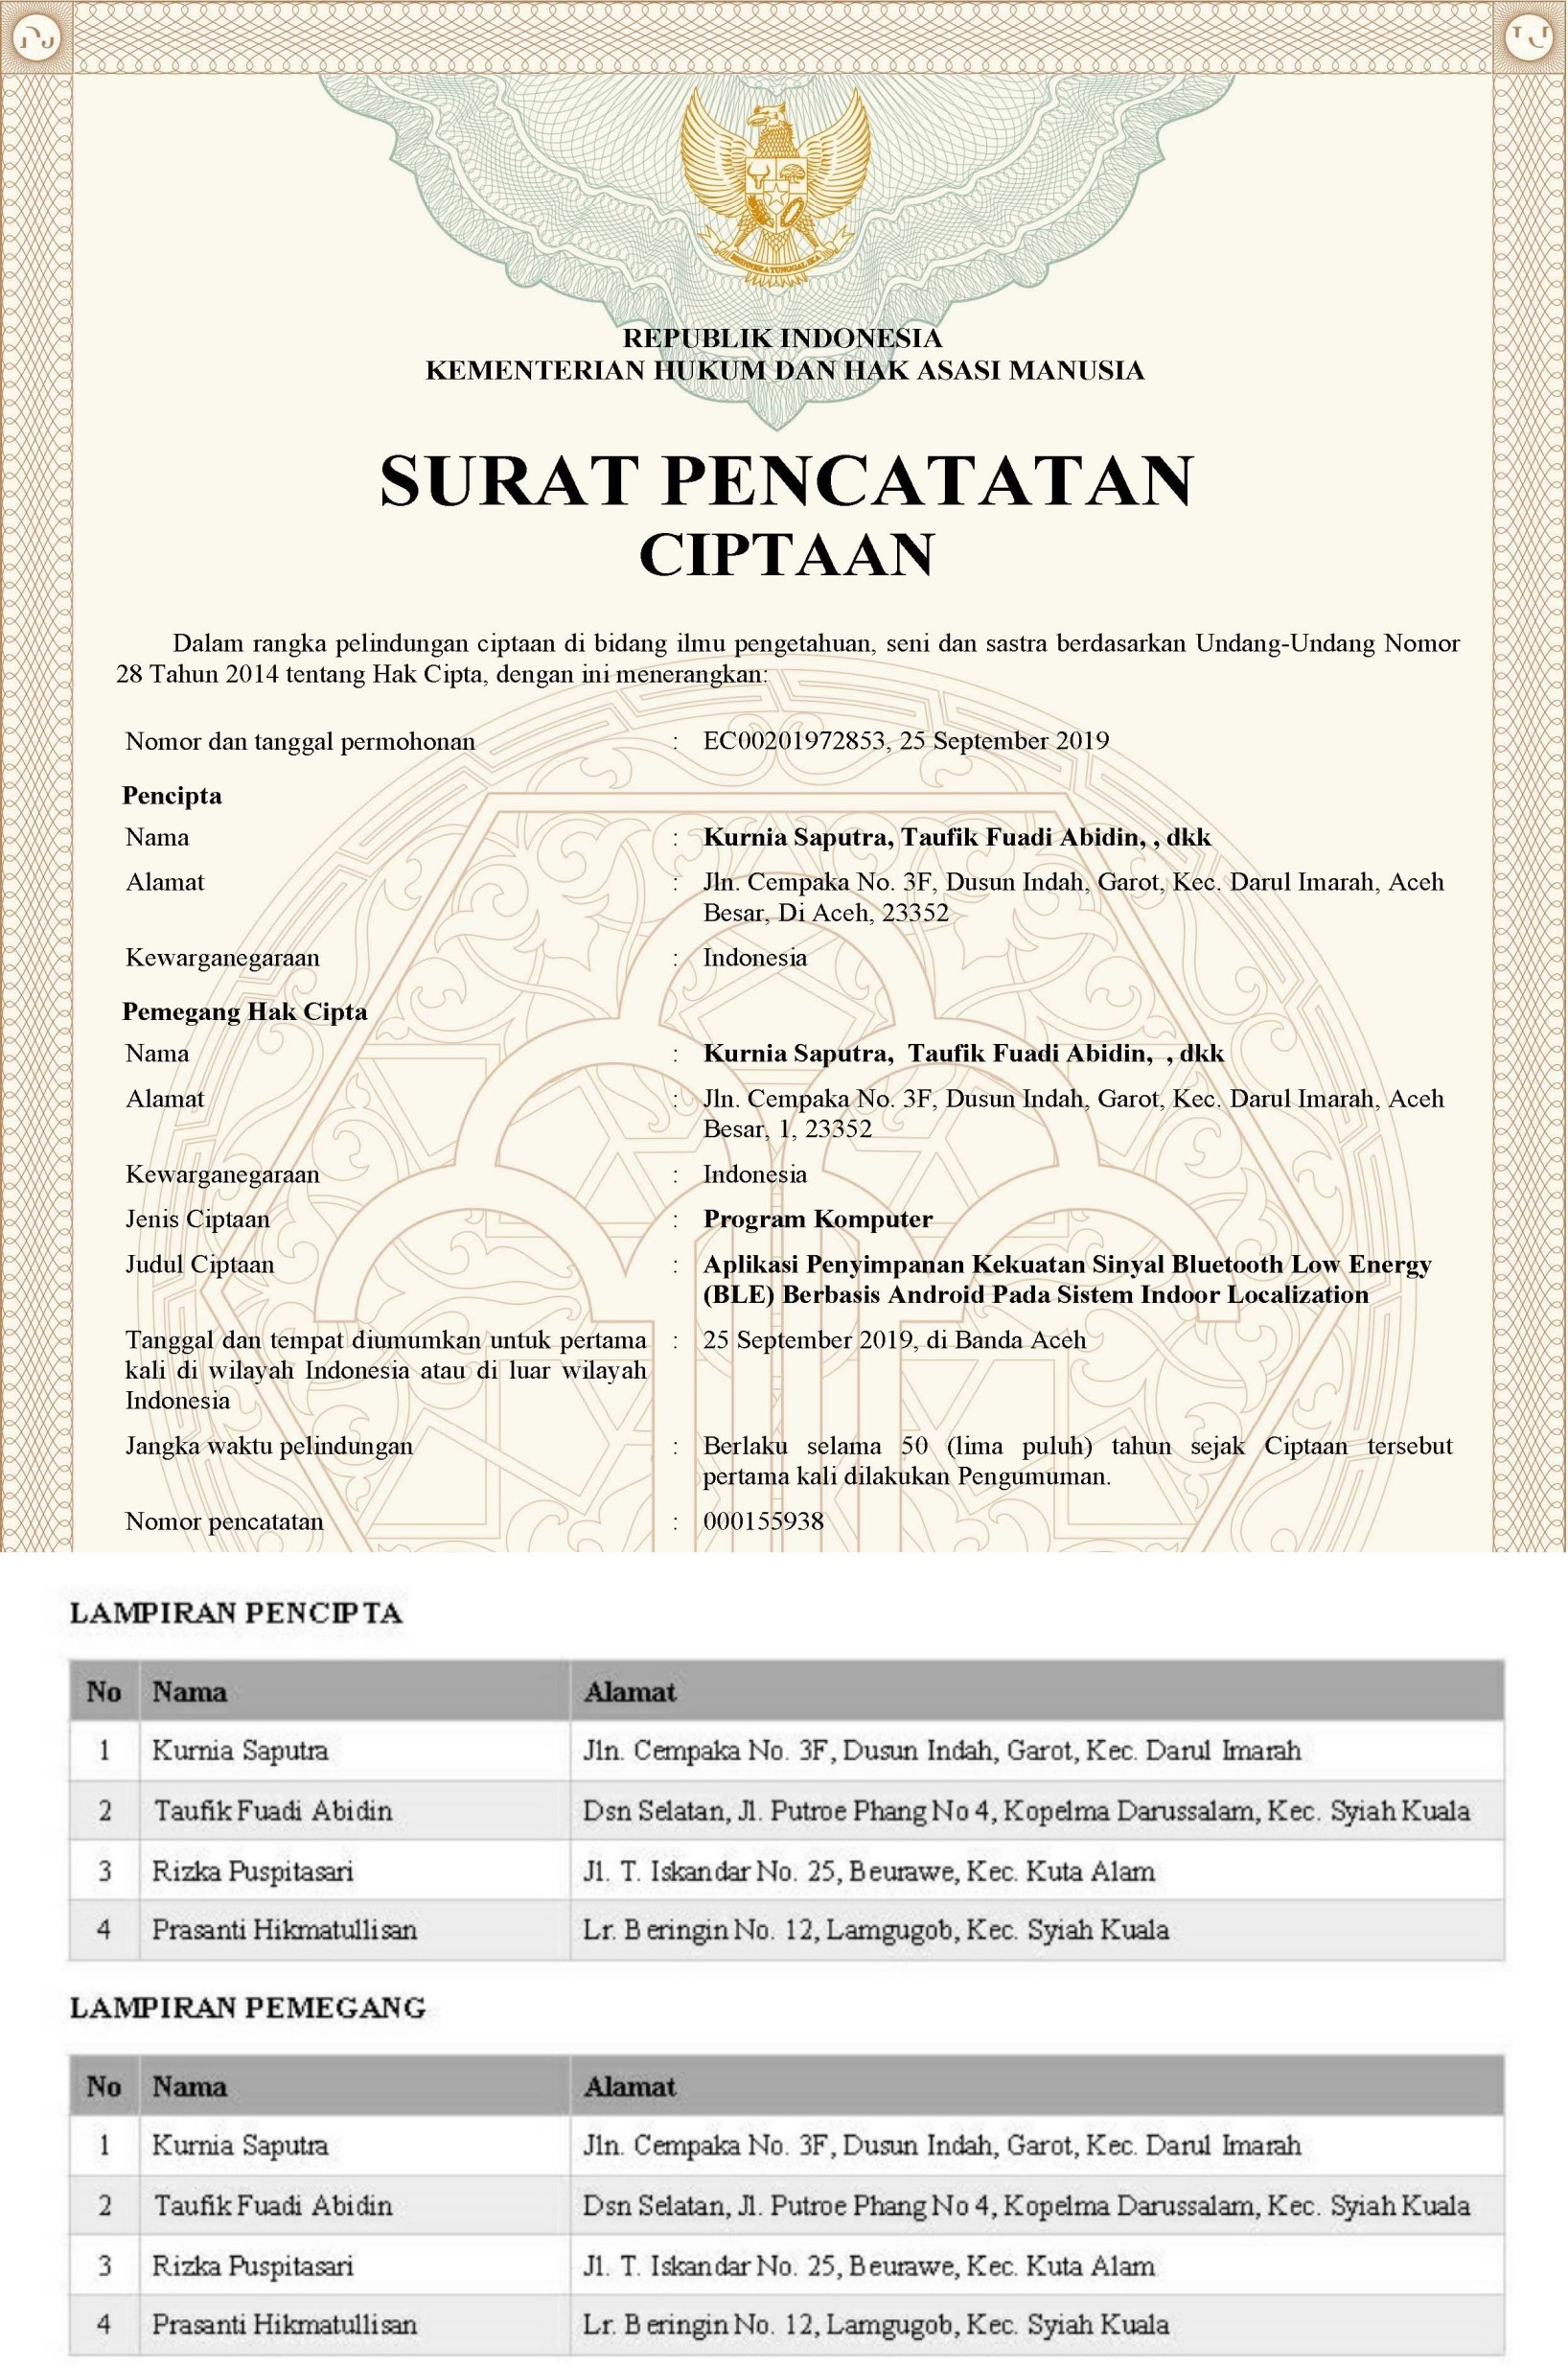
\includegraphics[width = 14cm, height = 21cm]{gambar/lampiran/sertifikat}
% \end{figure}

%------------------------------------------------------%
\addcontentsline{toc}{chapter}{LAMPIRAN 1}
\chapter*{Lampiran 1}
\newappendix{Lampiran 1. Foto Dokumentasi Proses \textit{Mapping}}
\begin{figure}[htp]
  \centering
  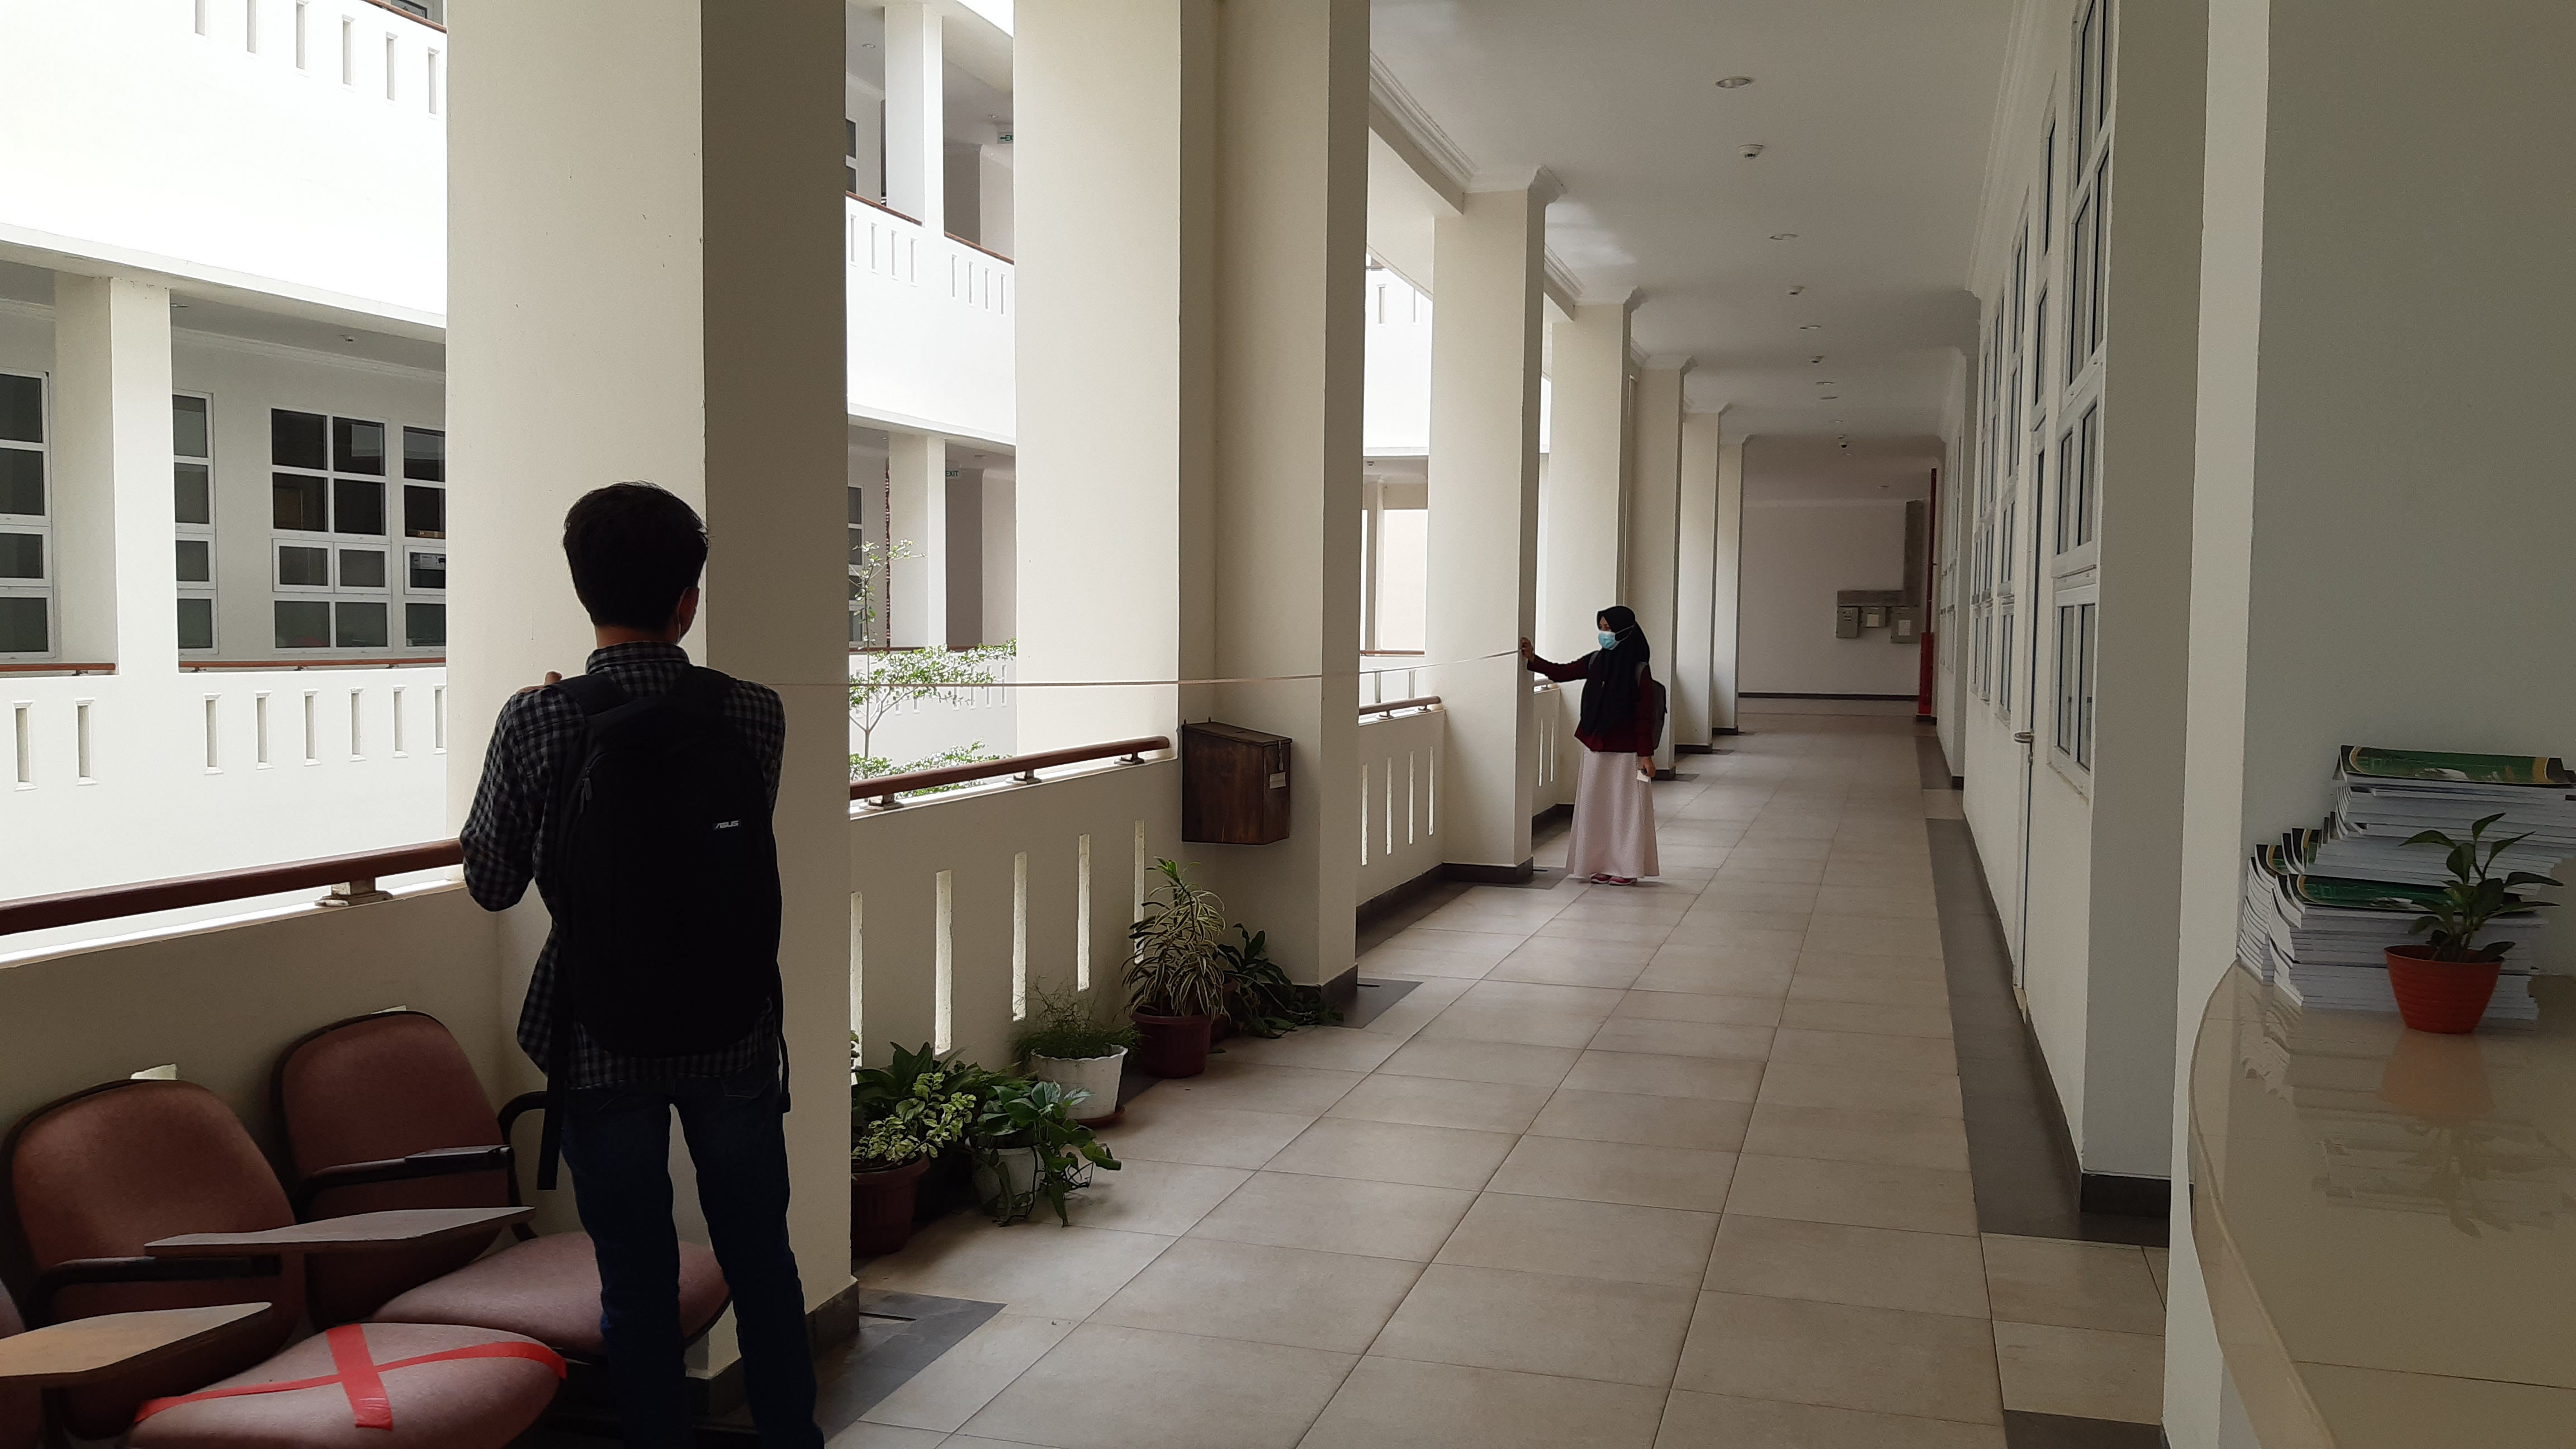
\includegraphics[width=.4\textwidth]{gambar/lampiran/lamp1a.jpg}\quad
  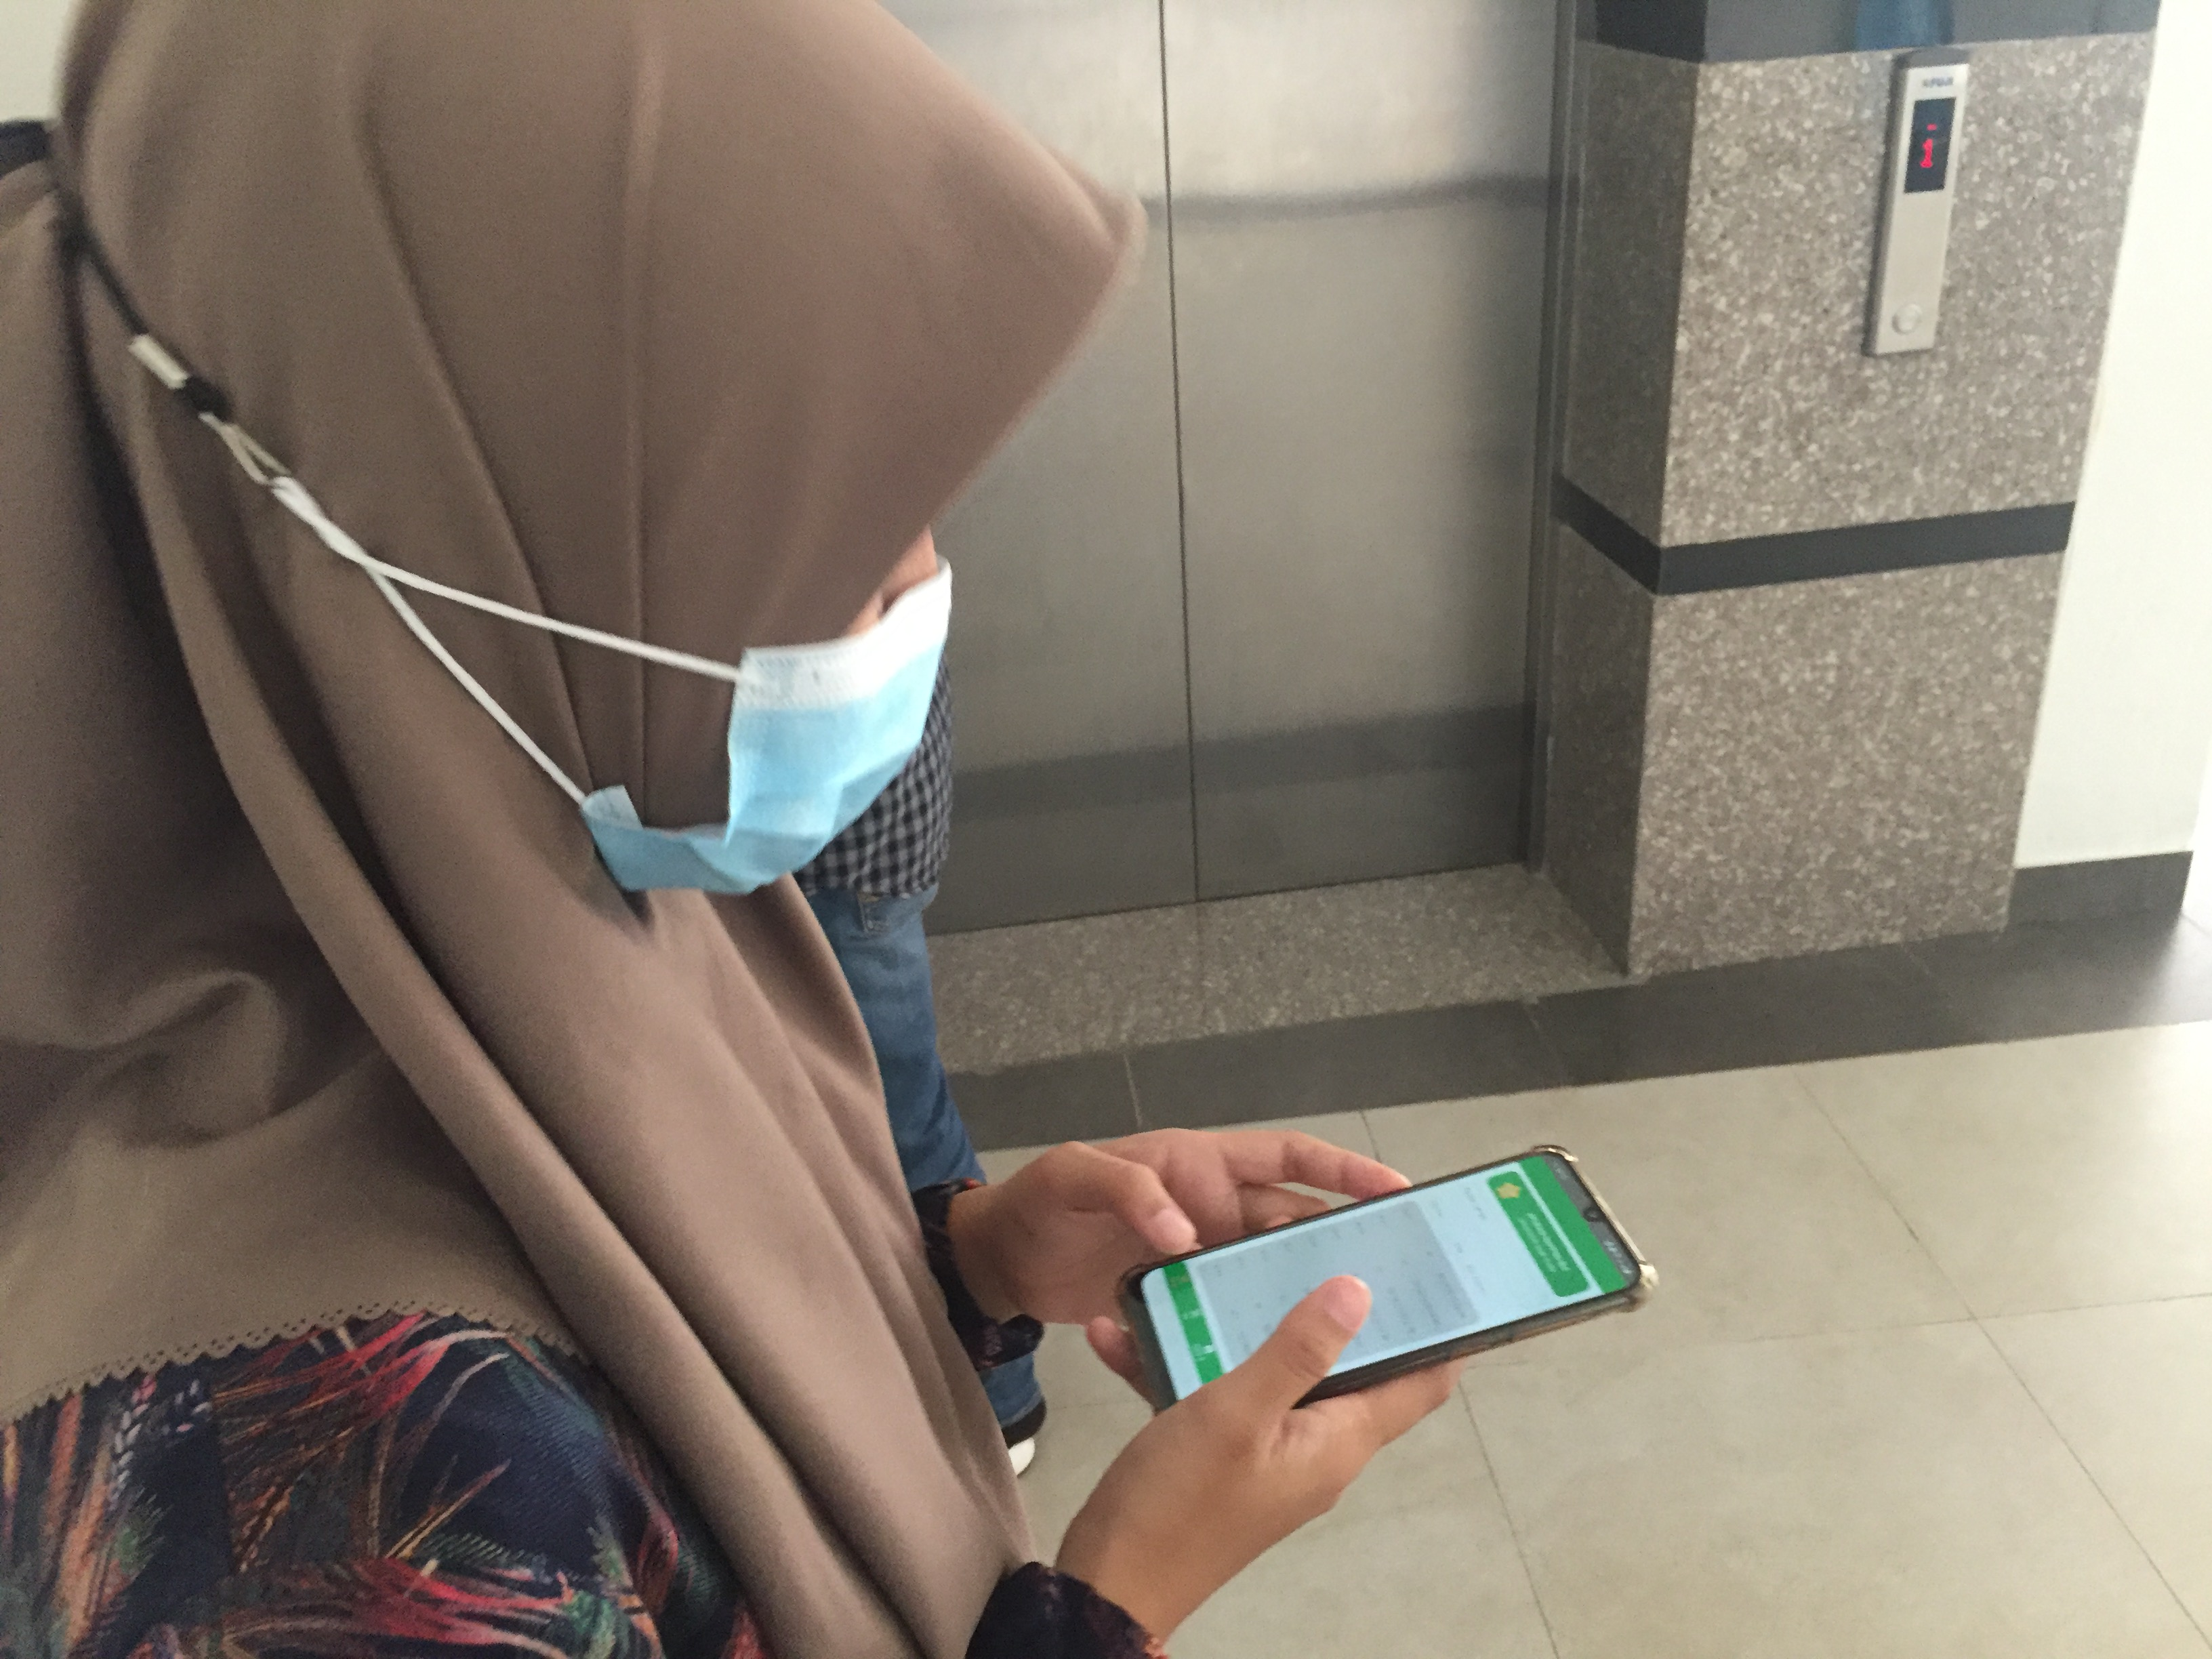
\includegraphics[width=.4\textwidth]{gambar/lampiran/lamp1d.jpg}\quad
  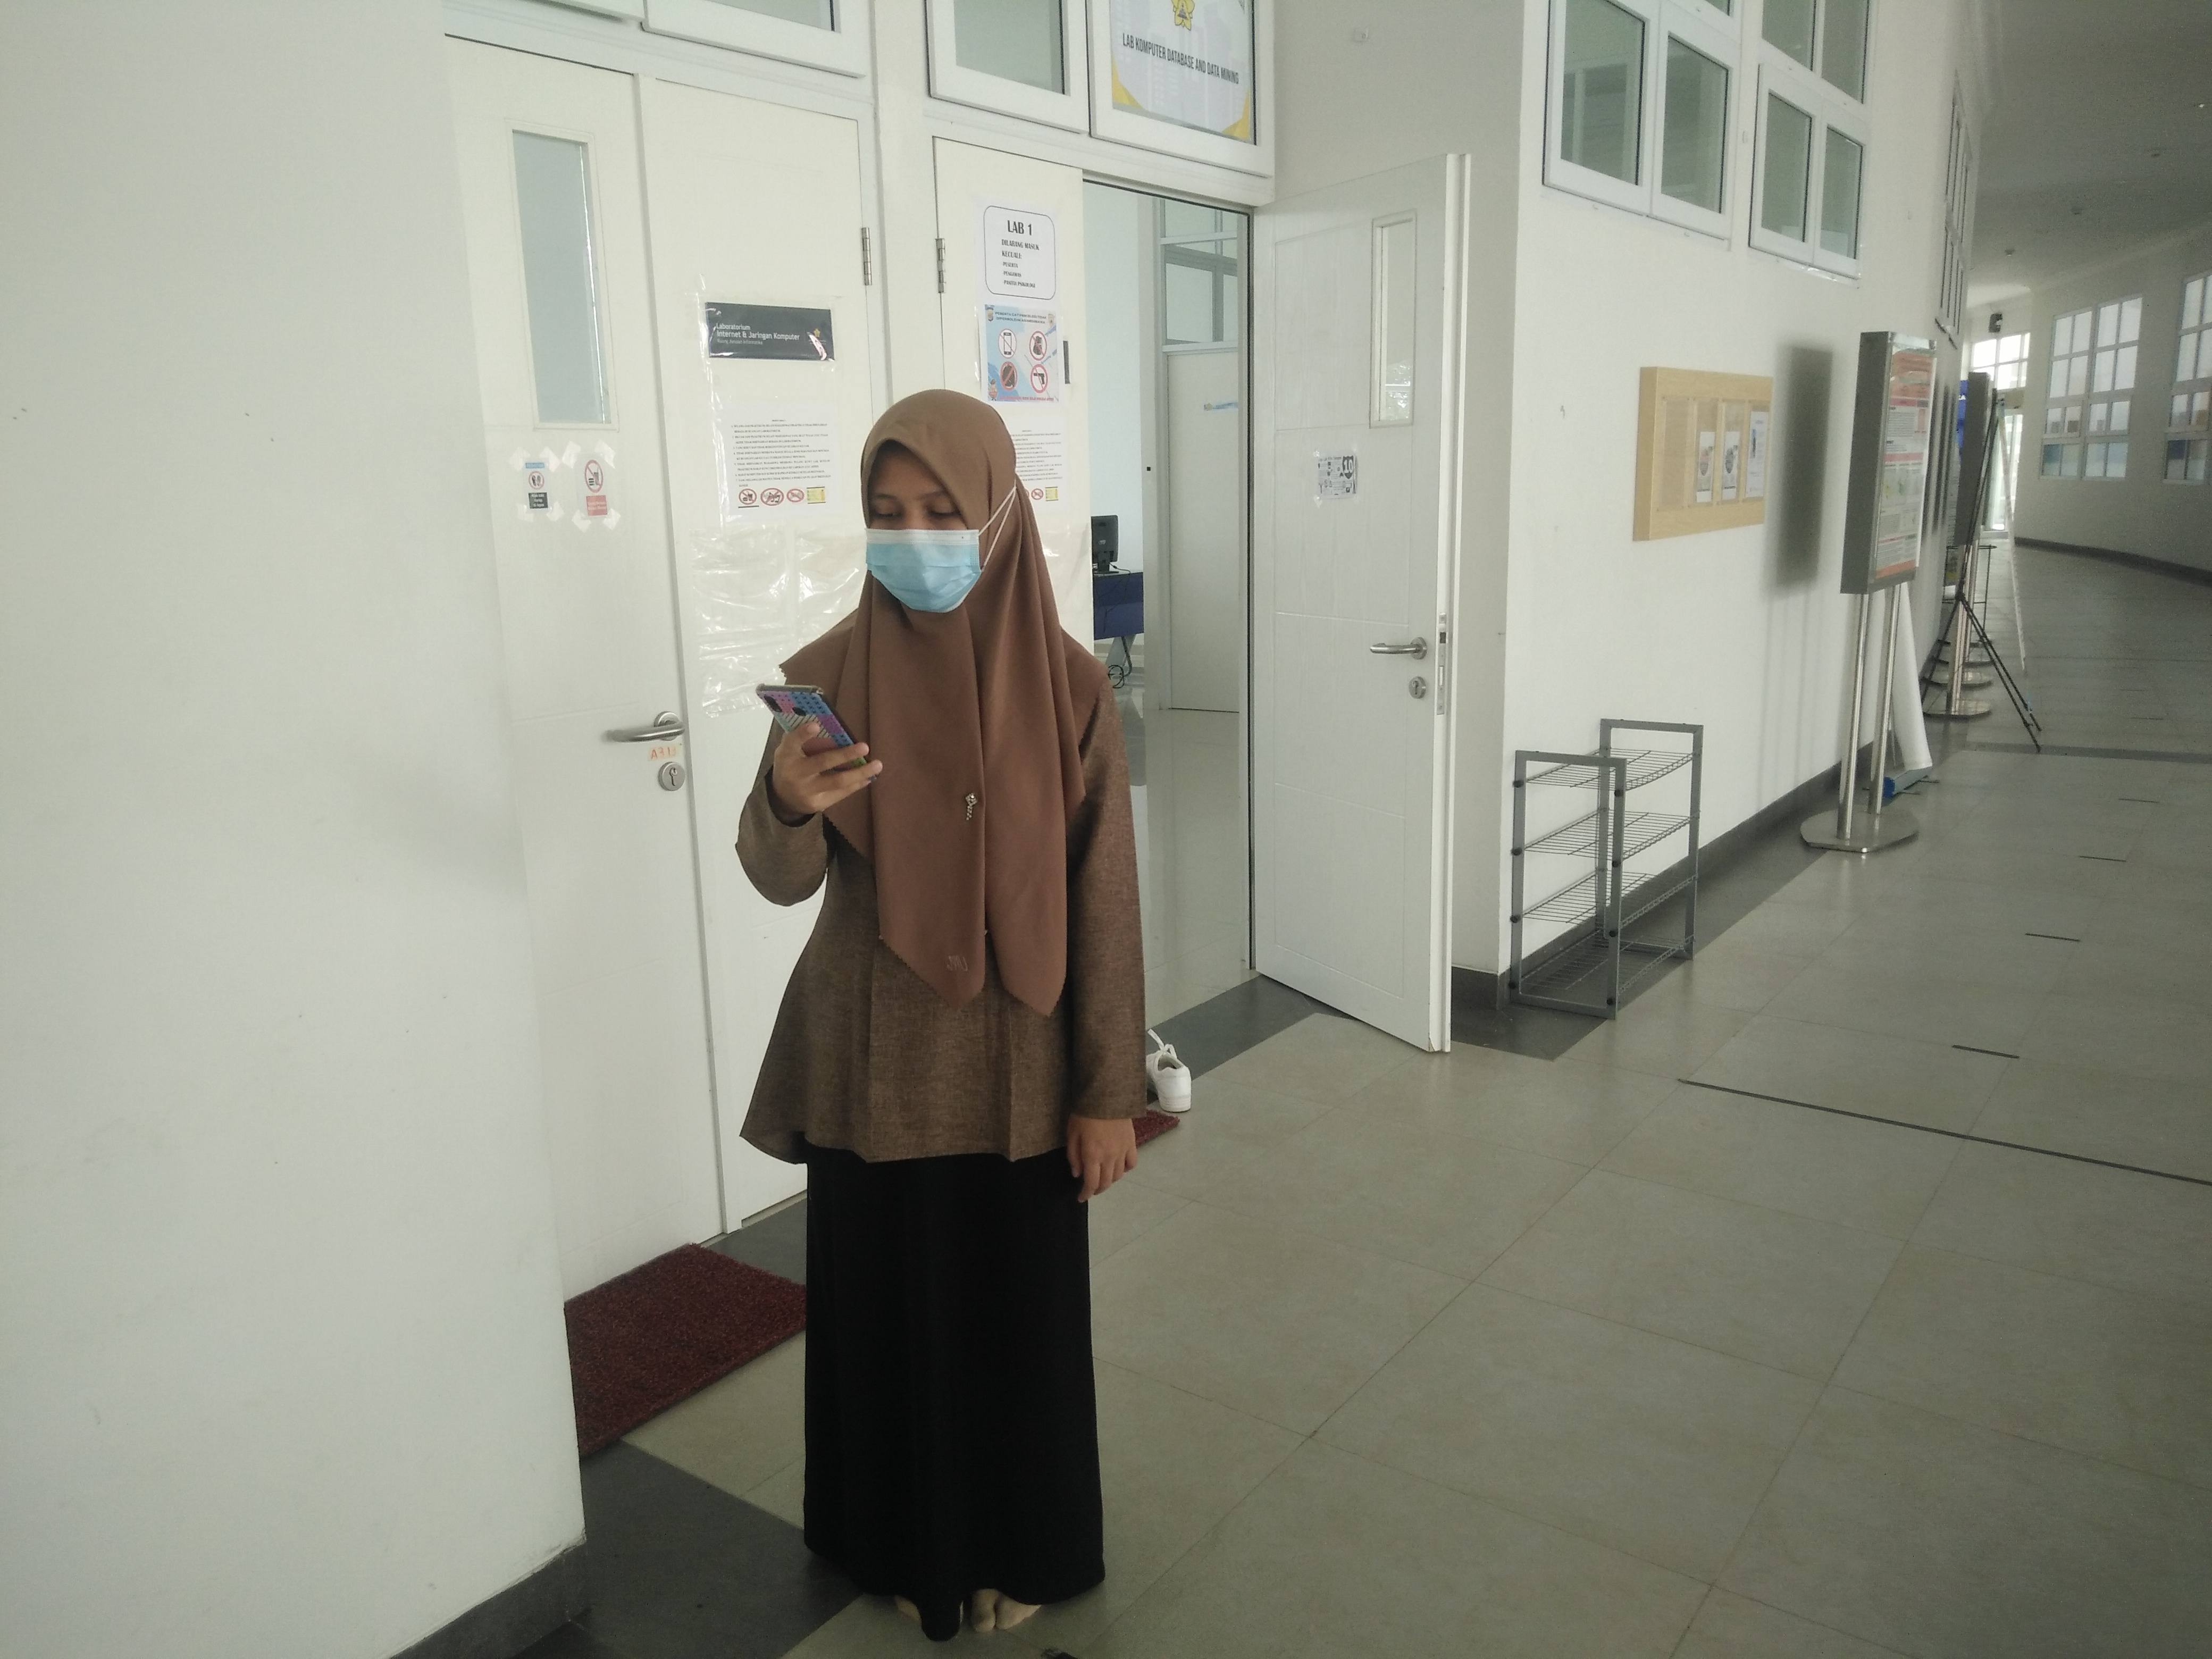
\includegraphics[width=.4\textwidth]{gambar/lampiran/lamp1f.jpg}

  \medskip

  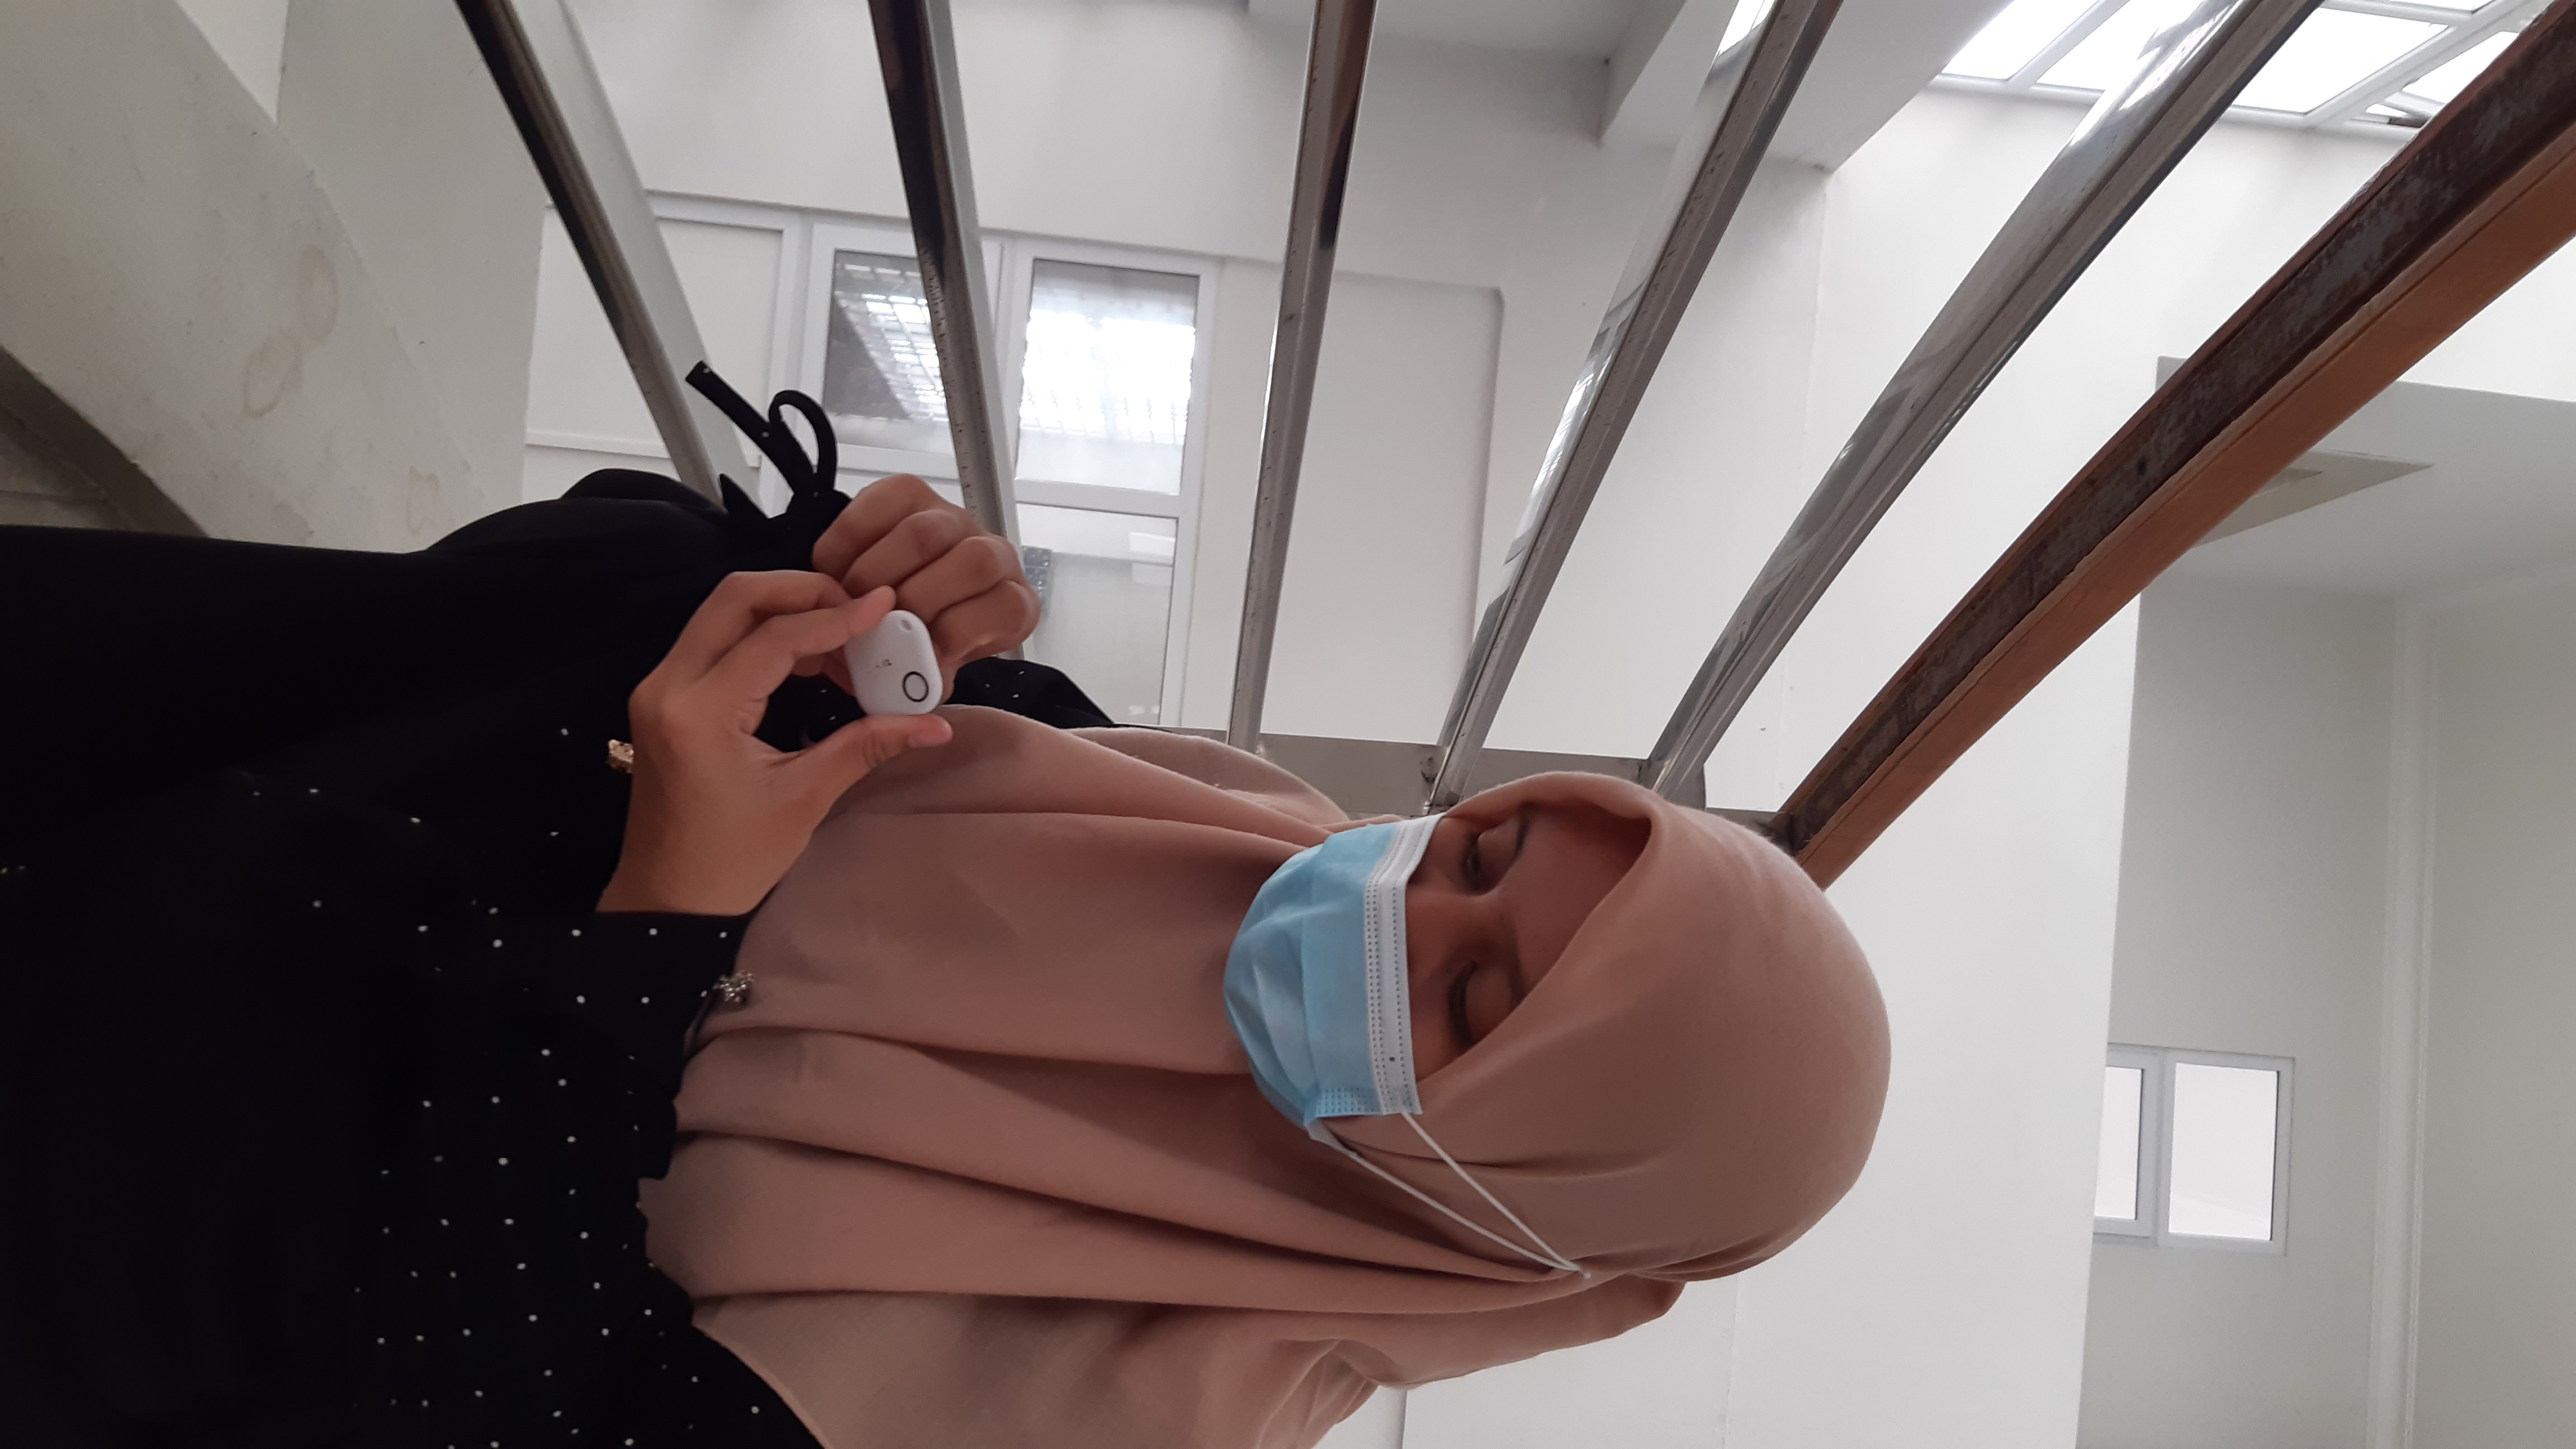
\includegraphics[width=.4\textwidth]{gambar/lampiran/lamp1b.JPG}\quad
  % 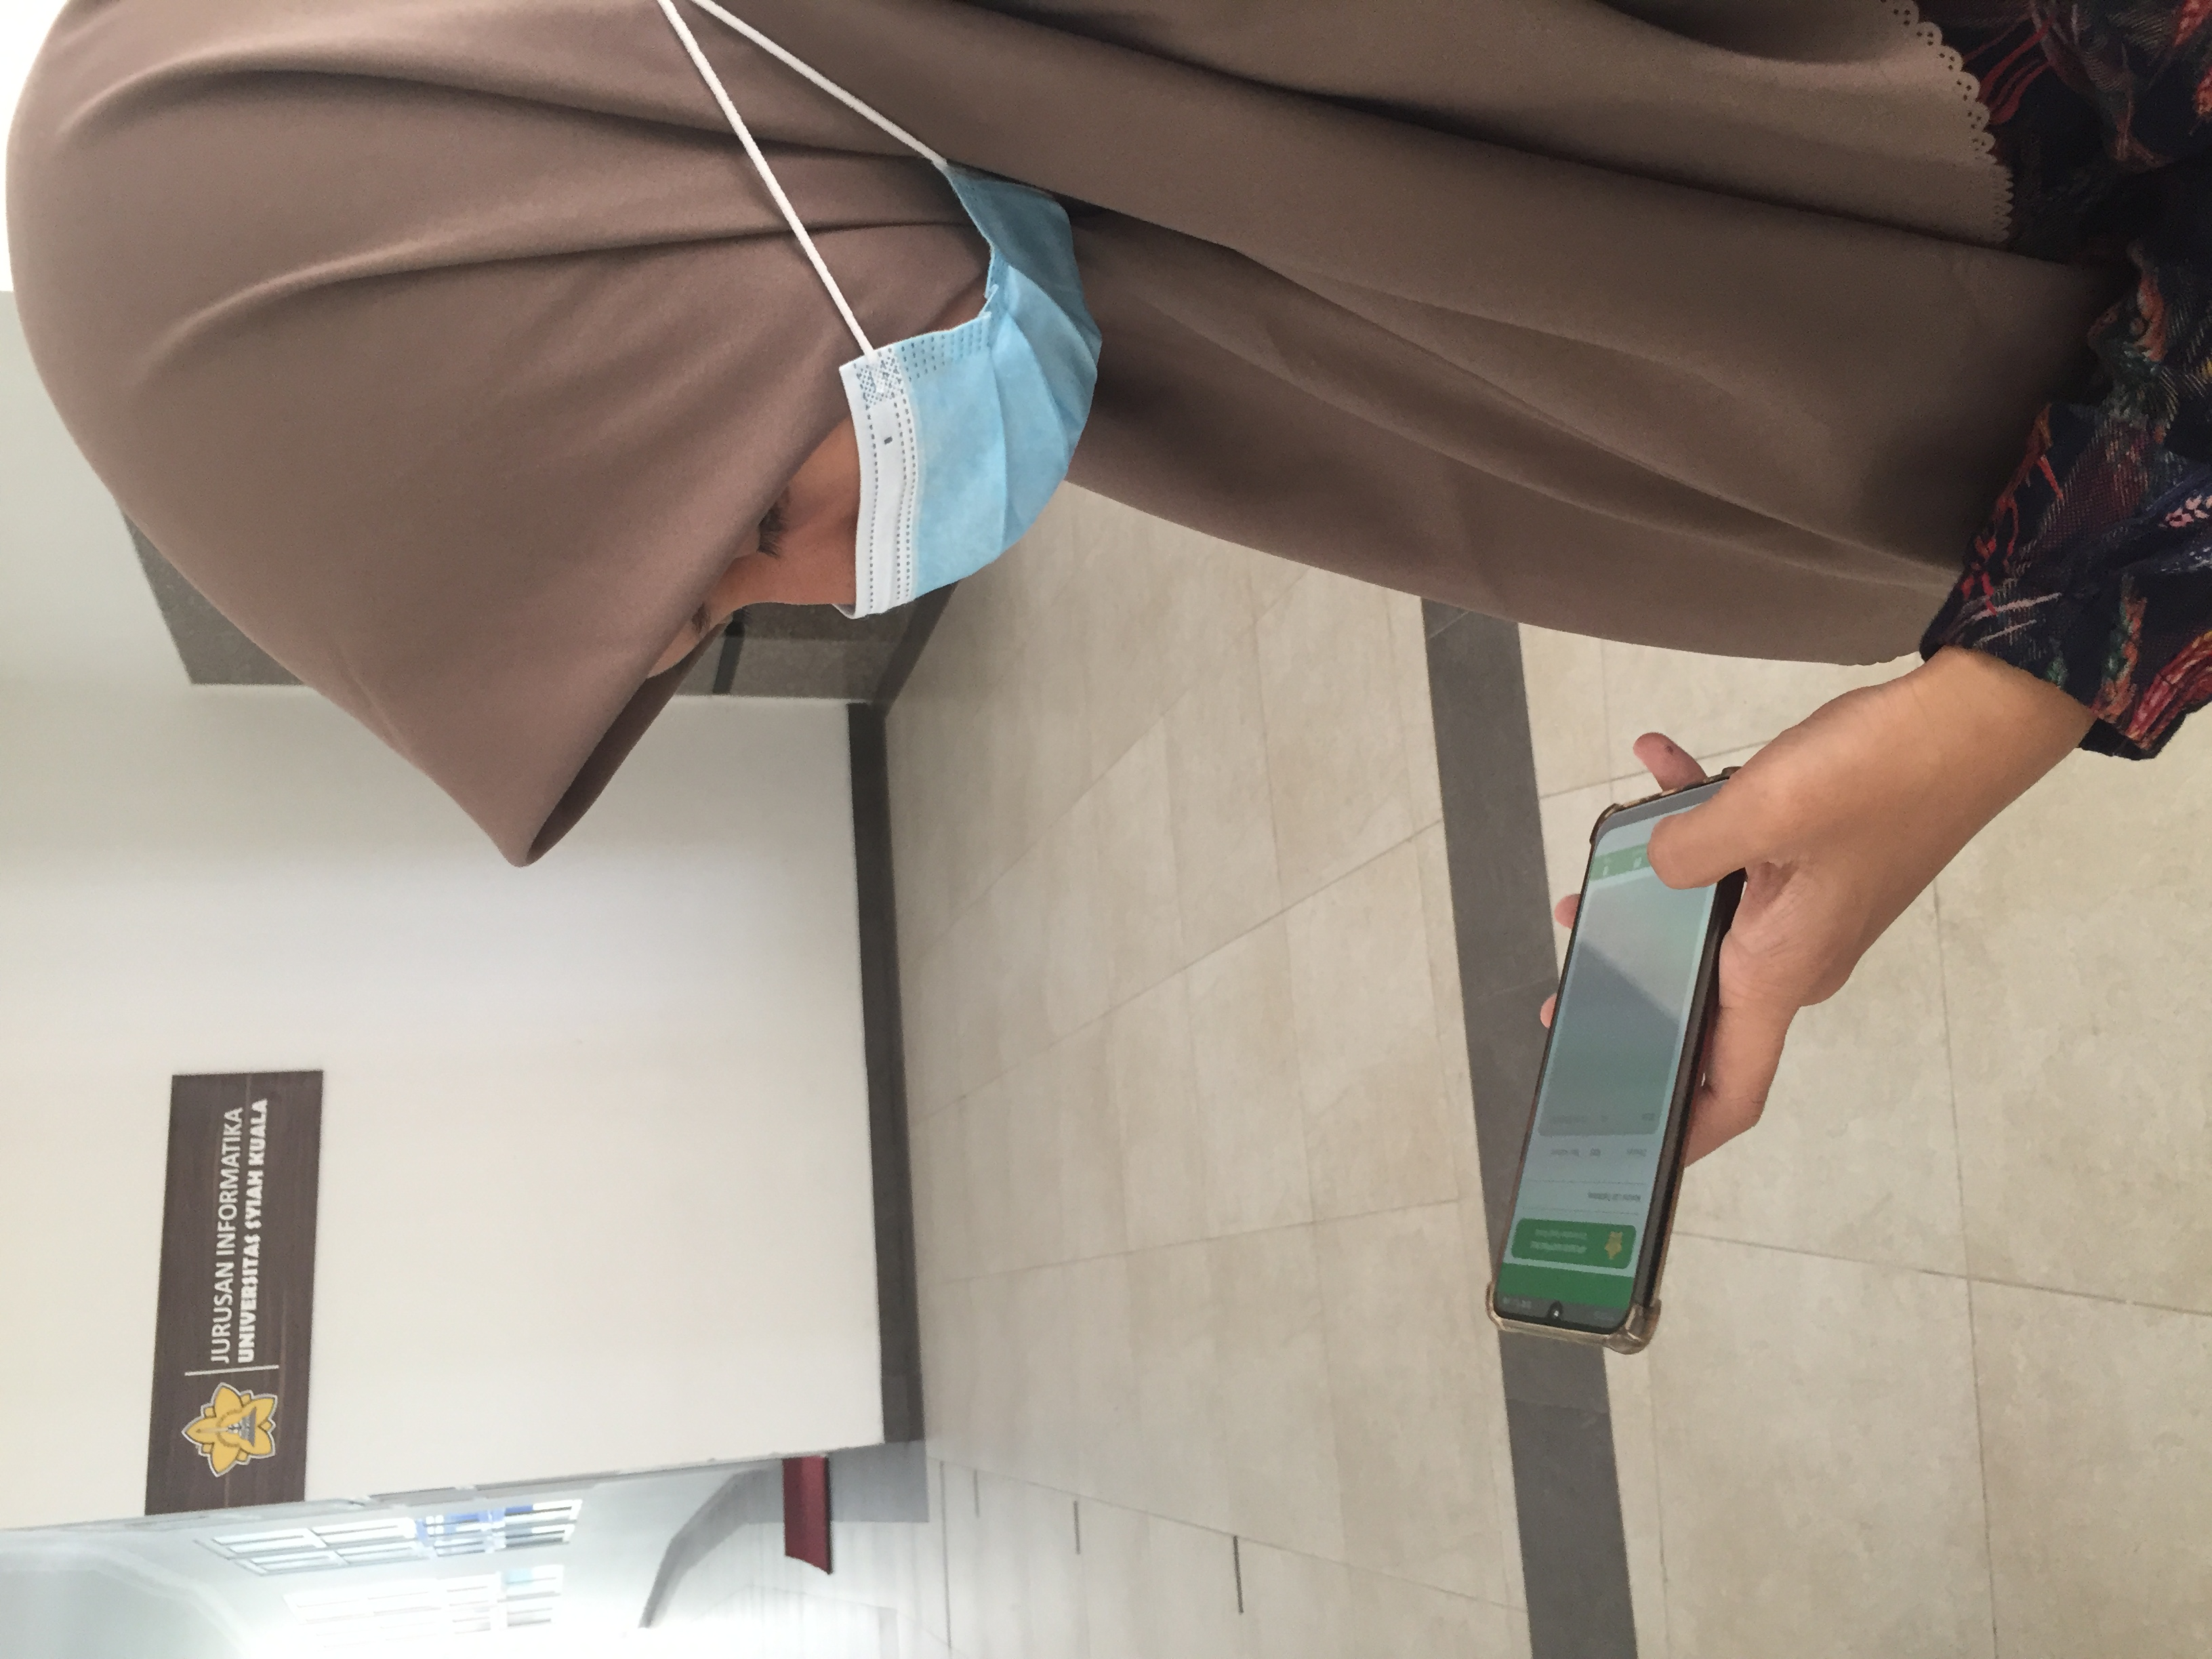
\includegraphics[width=.3\textwidth]{gambar/lampiran/lamp1e.JPG}
  \includegraphics[width=.4\textwidth]{gambar/lampiran/lamp1c.JPG}
  \label{sus-dosen}
\end{figure}


\vspace{2cm}




%-----------------------------------------------------------------------------%
\addcontentsline{toc}{chapter}{LAMPIRAN 2}
\chapter*{Lampiran 2}
\newappendix{Lampiran 2. Foto Dokumentasi Proses Pengujian x \textit{Usability}}
\begin{figure}[htp]
  \centering
  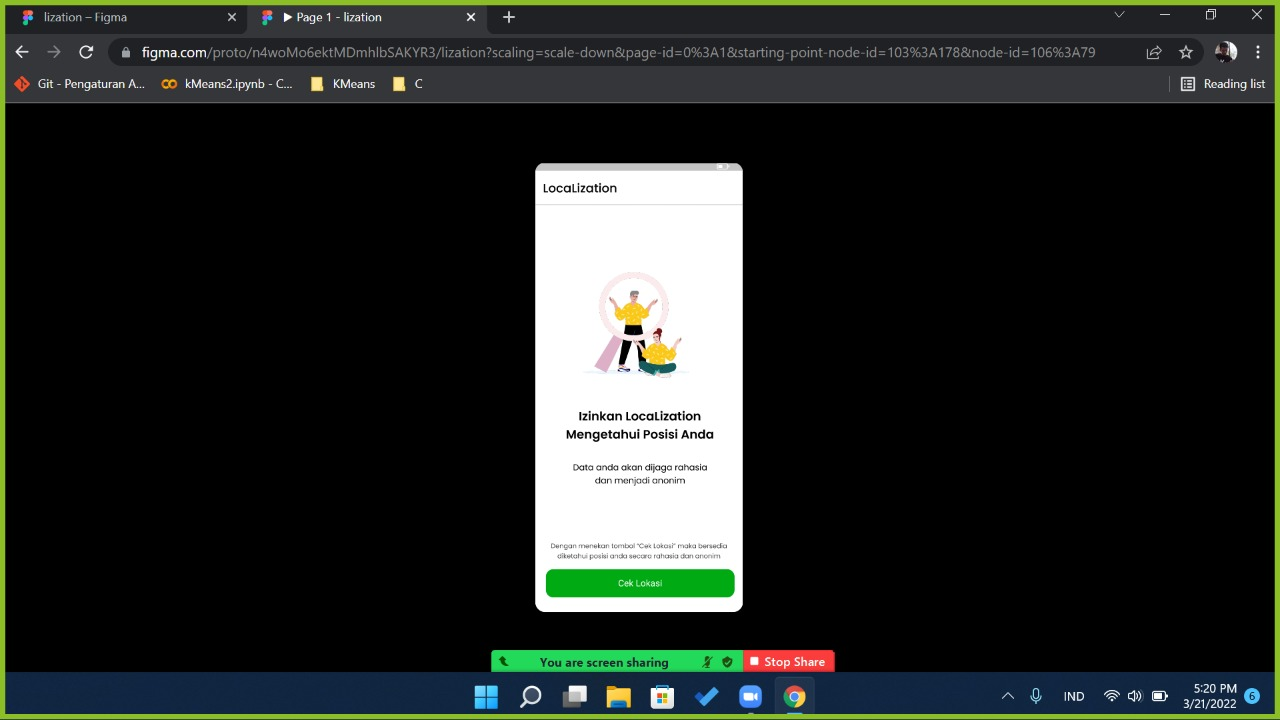
\includegraphics[width=.4\textwidth]{gambar/lampiran/umux1.jpeg}\quad
  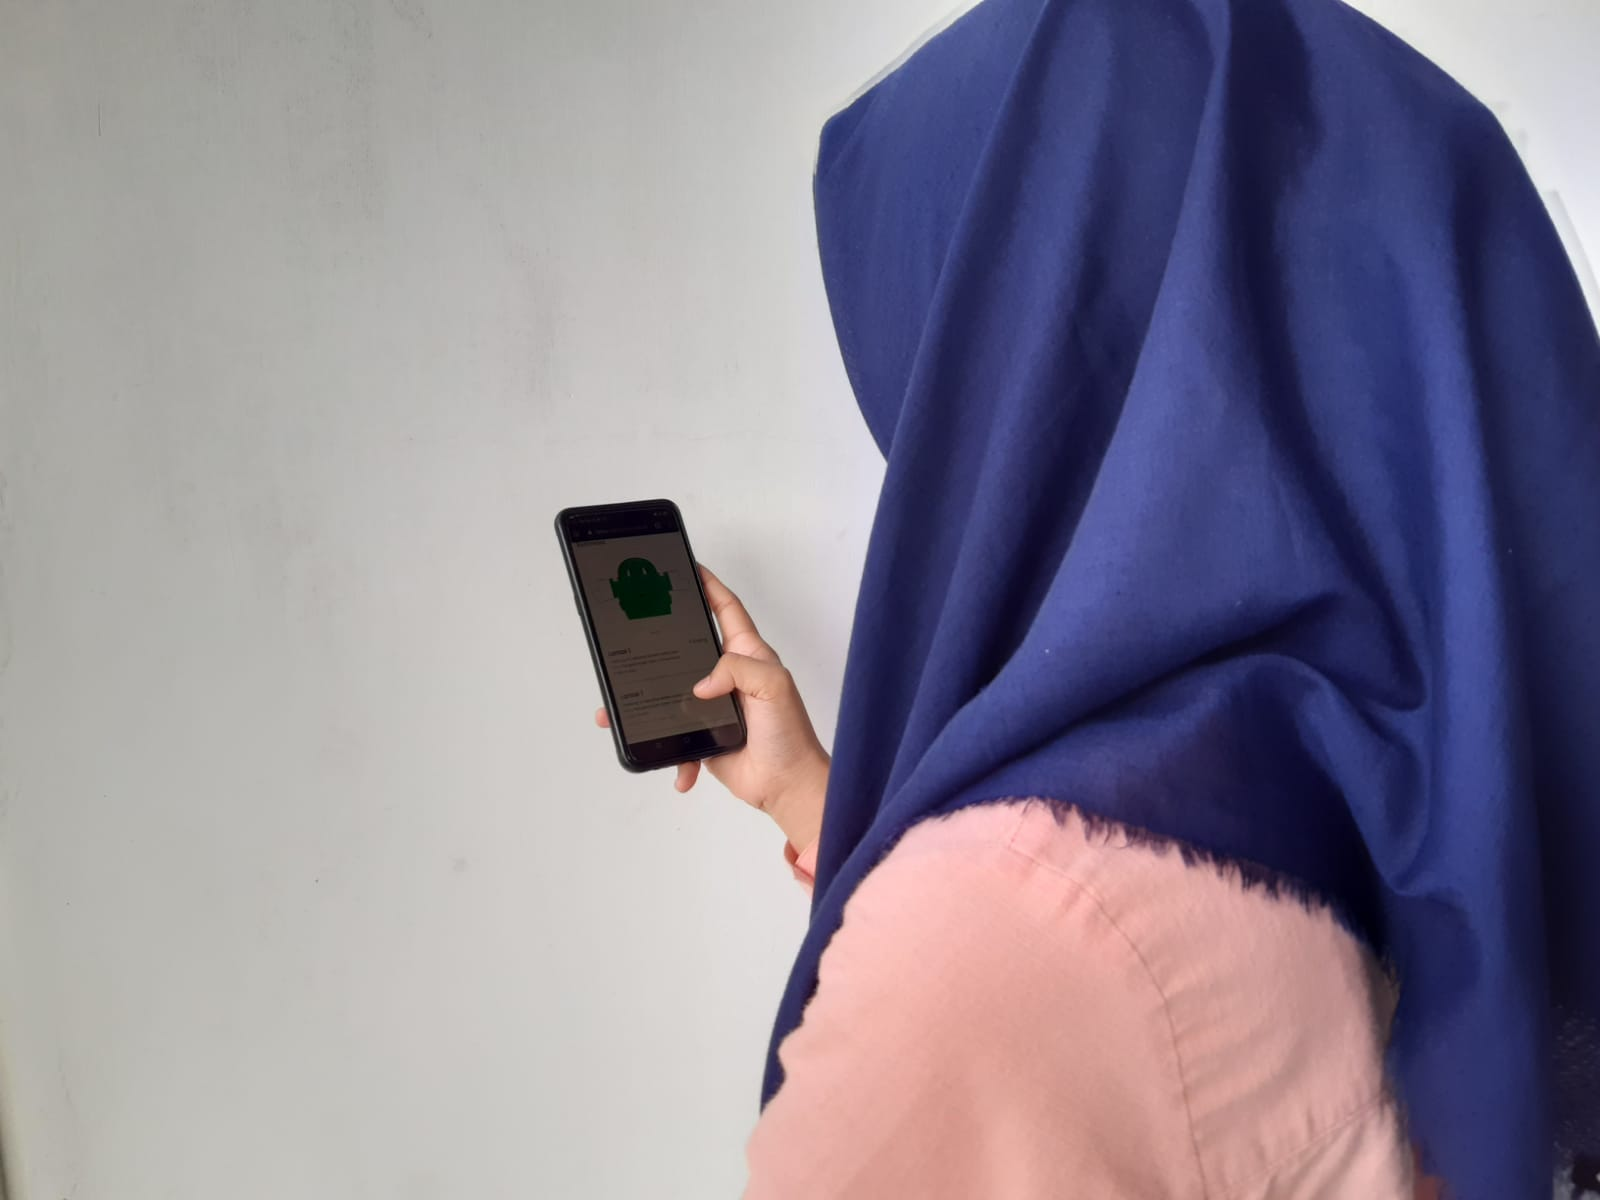
\includegraphics[width=.4\textwidth]{gambar/lampiran/umux2.jpeg}\quad
  % 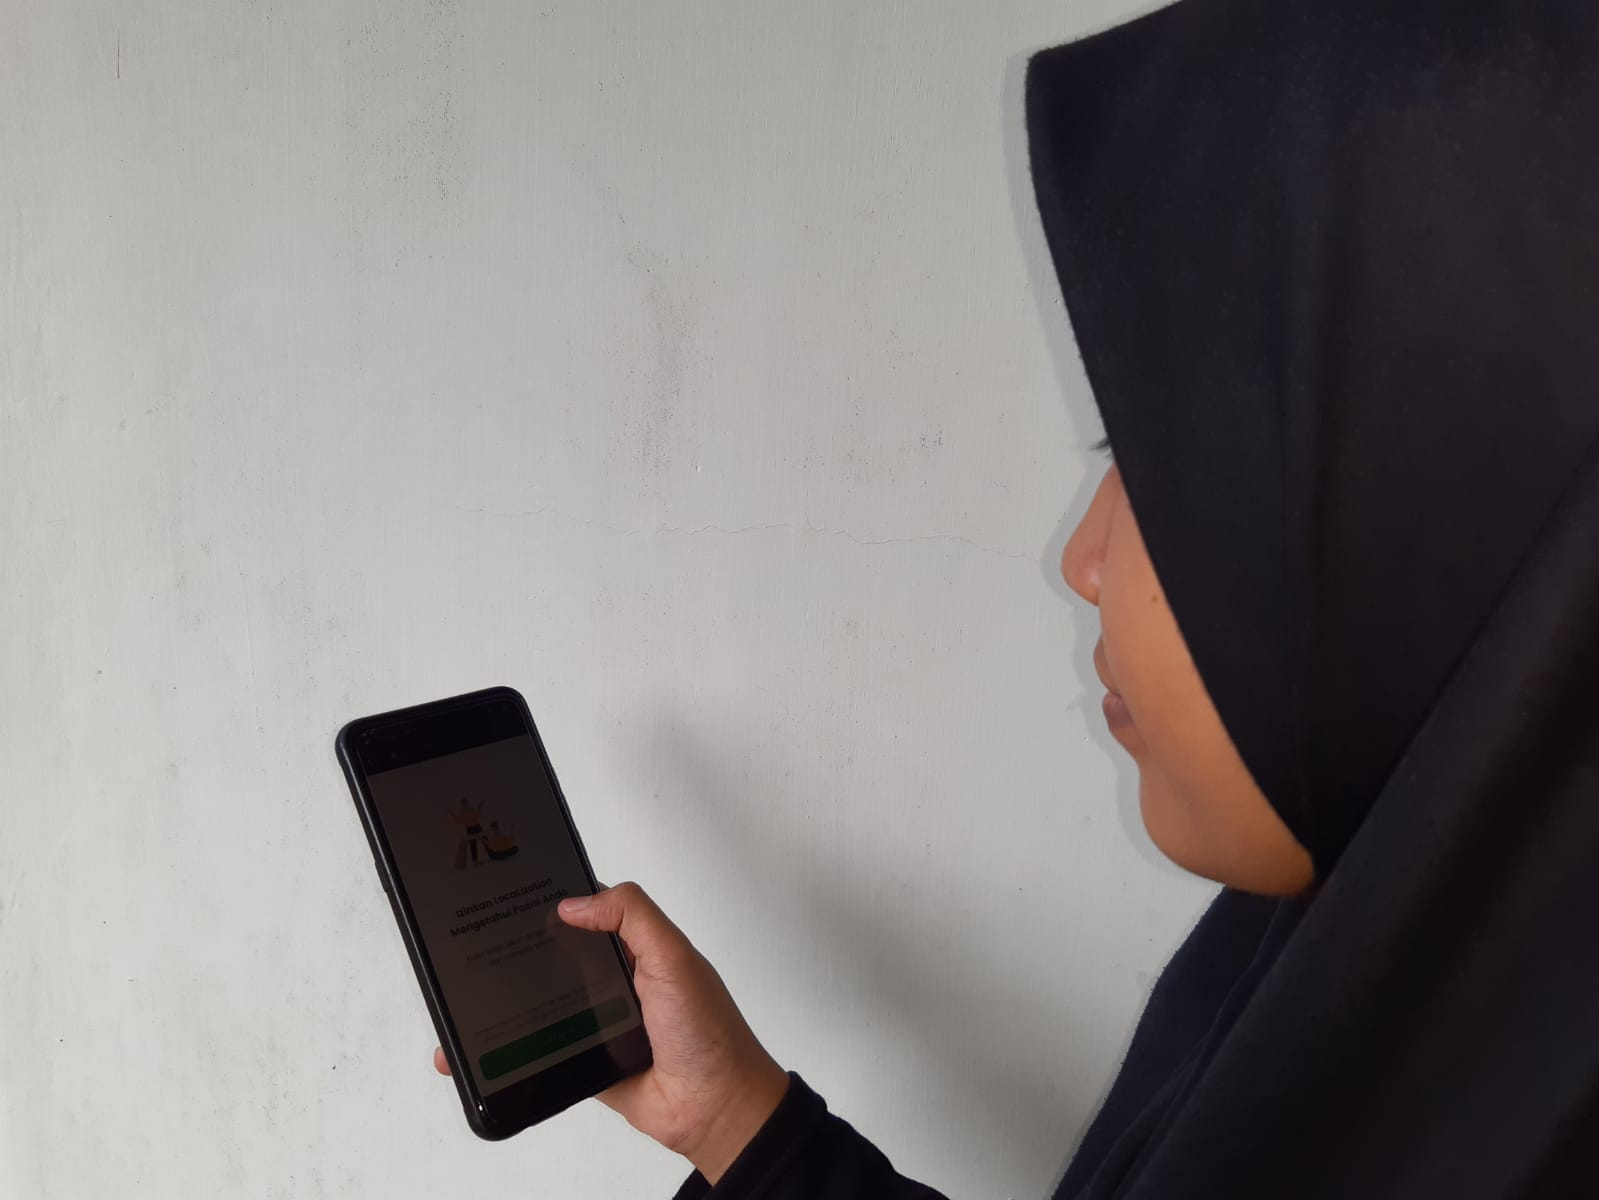
\includegraphics[width=.3\textwidth]{gambar/lampiran/umux3.jpeg}

  \medskip

  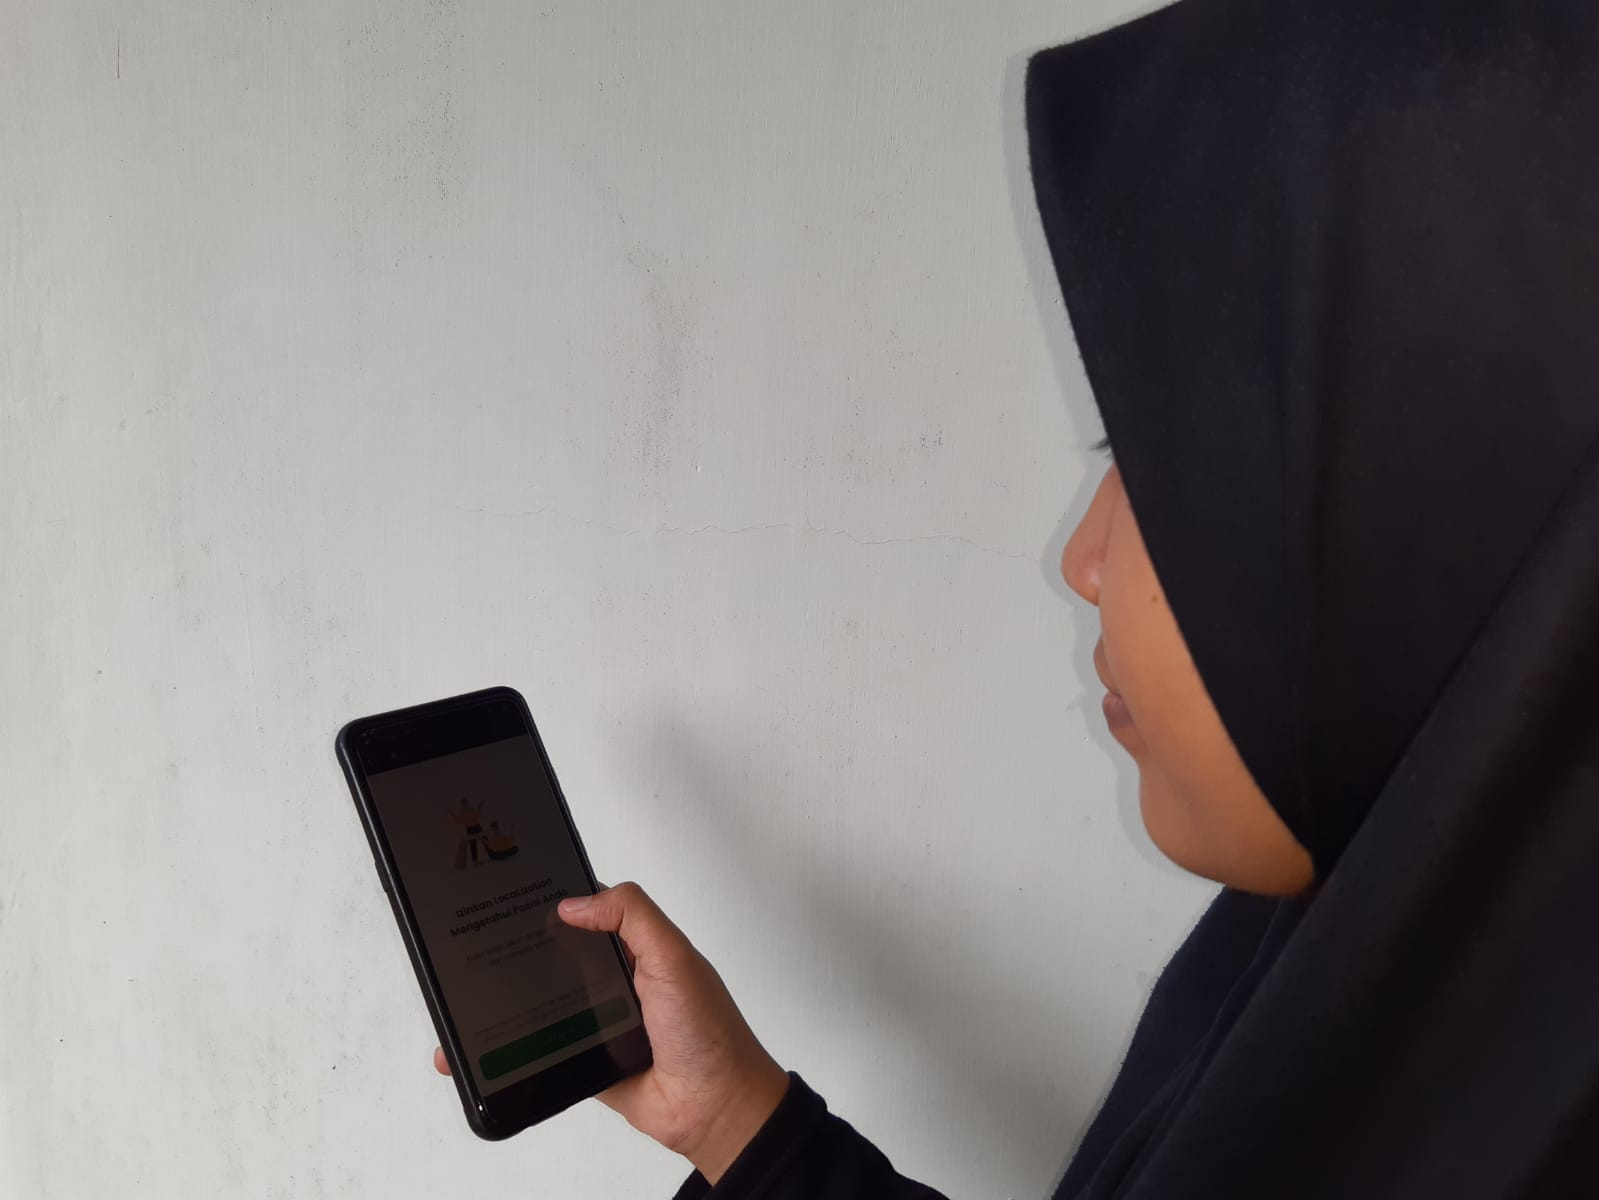
\includegraphics[width=.4\textwidth]{gambar/lampiran/umux3.jpeg}\quad
  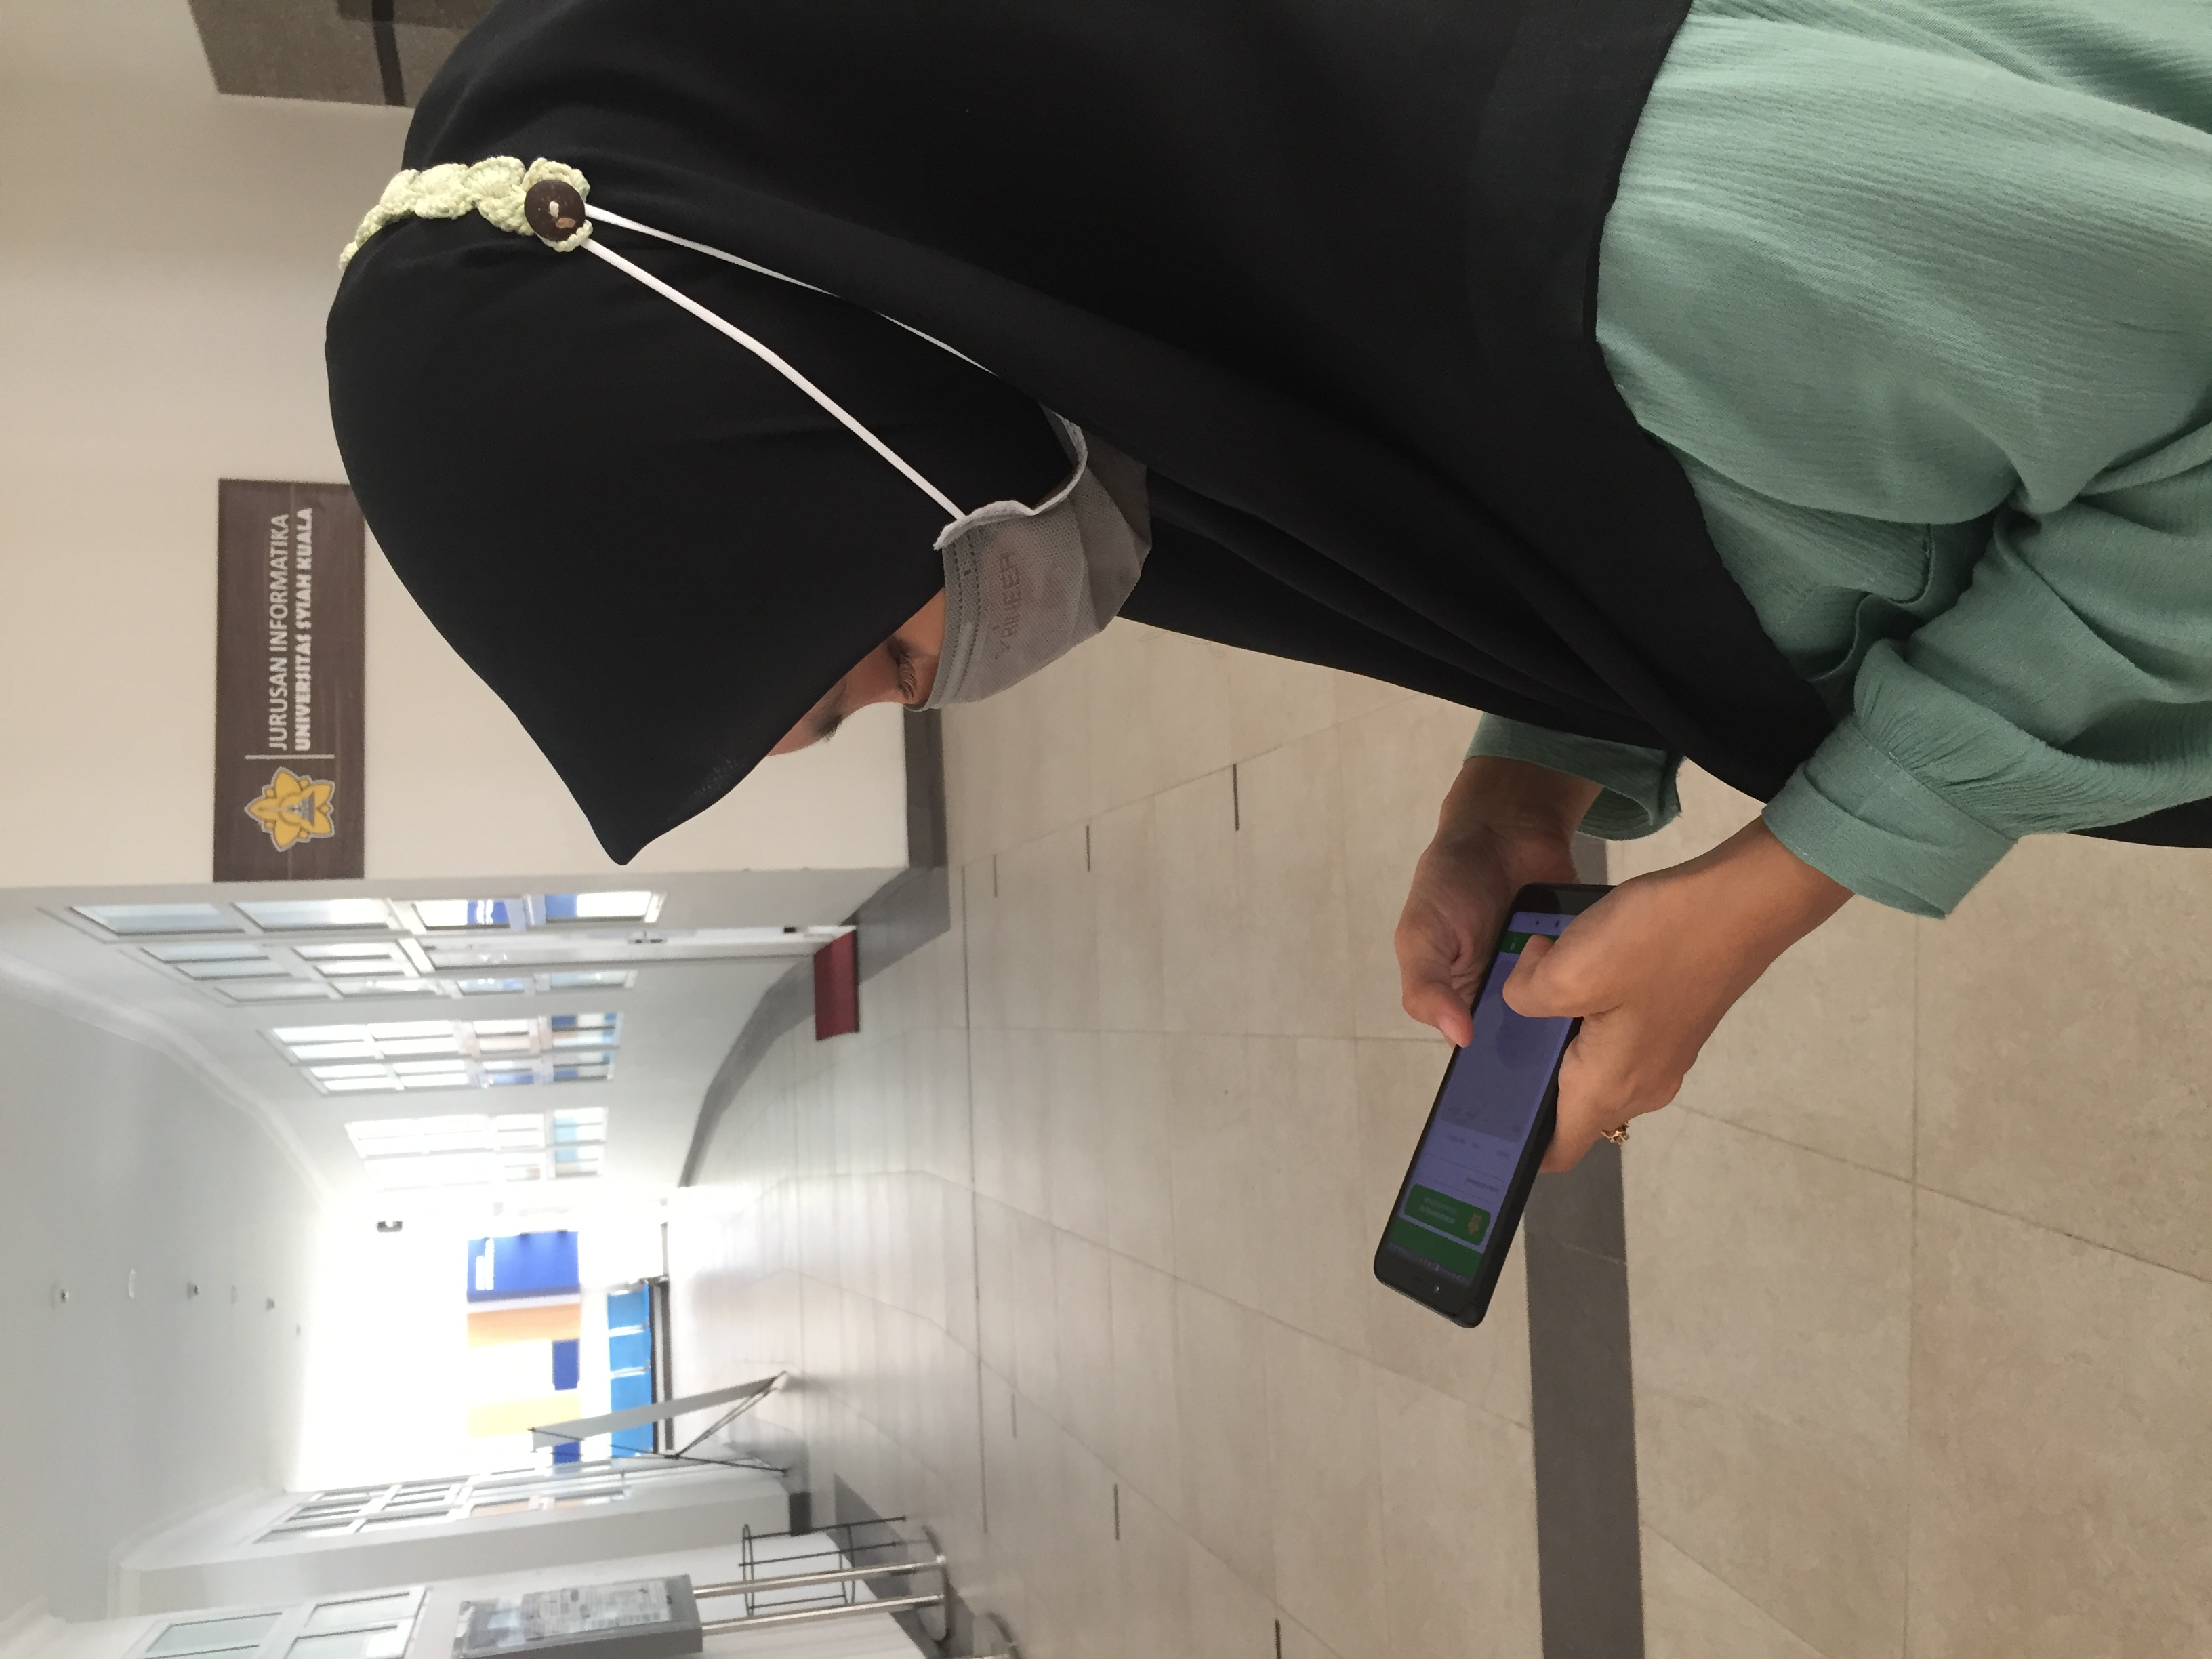
\includegraphics[width=.4\textwidth]{gambar/lampiran/umux4.JPG}

  \label{sus-mahasiswa}
\end{figure}
%-----------------------------------------------------------------------------%

\addcontentsline{toc}{chapter}{LAMPIRAN 3}
\chapter*{Lampiran 3}
\newappendix{Lampiran 3. Foto Dokumentasi Scrum}
\begin{figure}[htp]
  \centering
  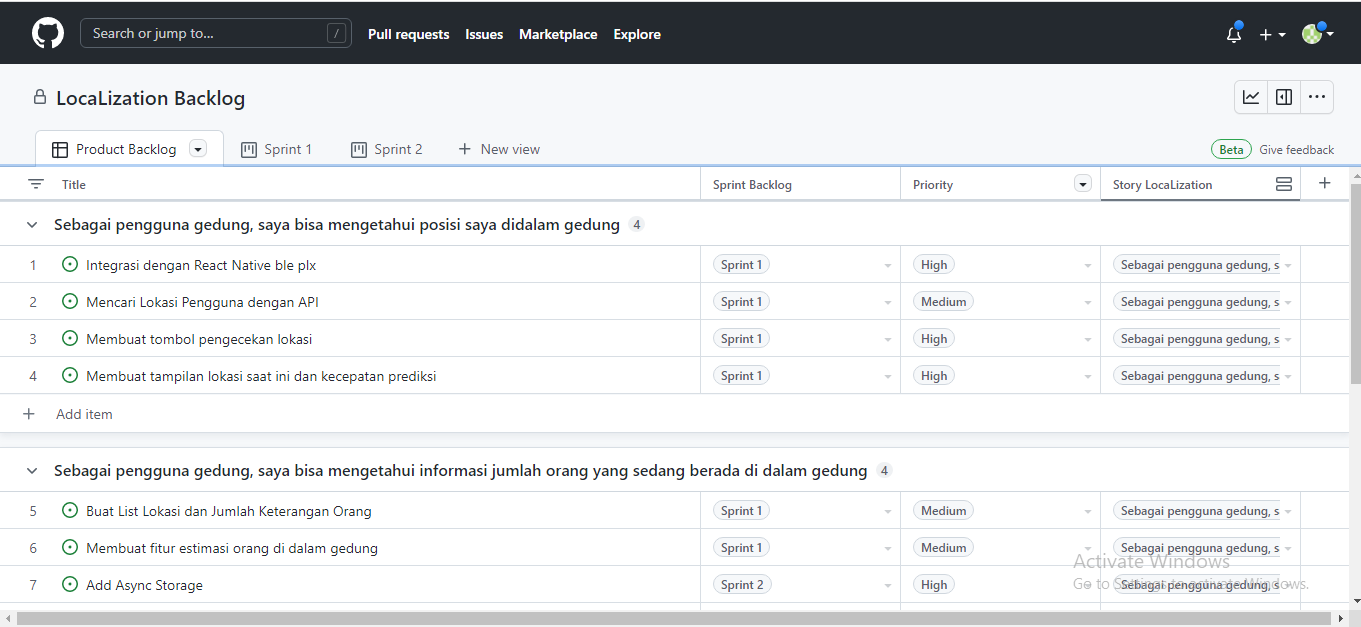
\includegraphics[width=.4\textwidth]{gambar/lampiran/scrum1.PNG}\quad
  \vspace{0.4cm}
  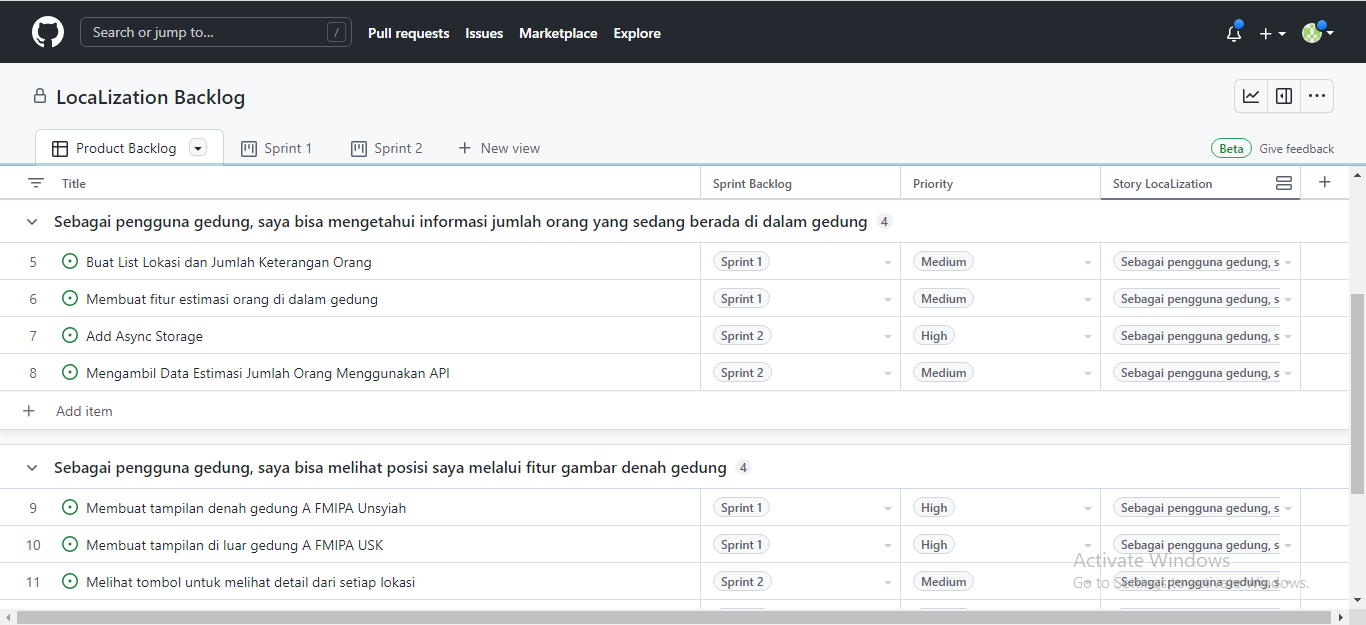
\includegraphics[width=.4\textwidth]{gambar/lampiran/scrum2.PNG}\quad
  \vspace{0.4cm}
  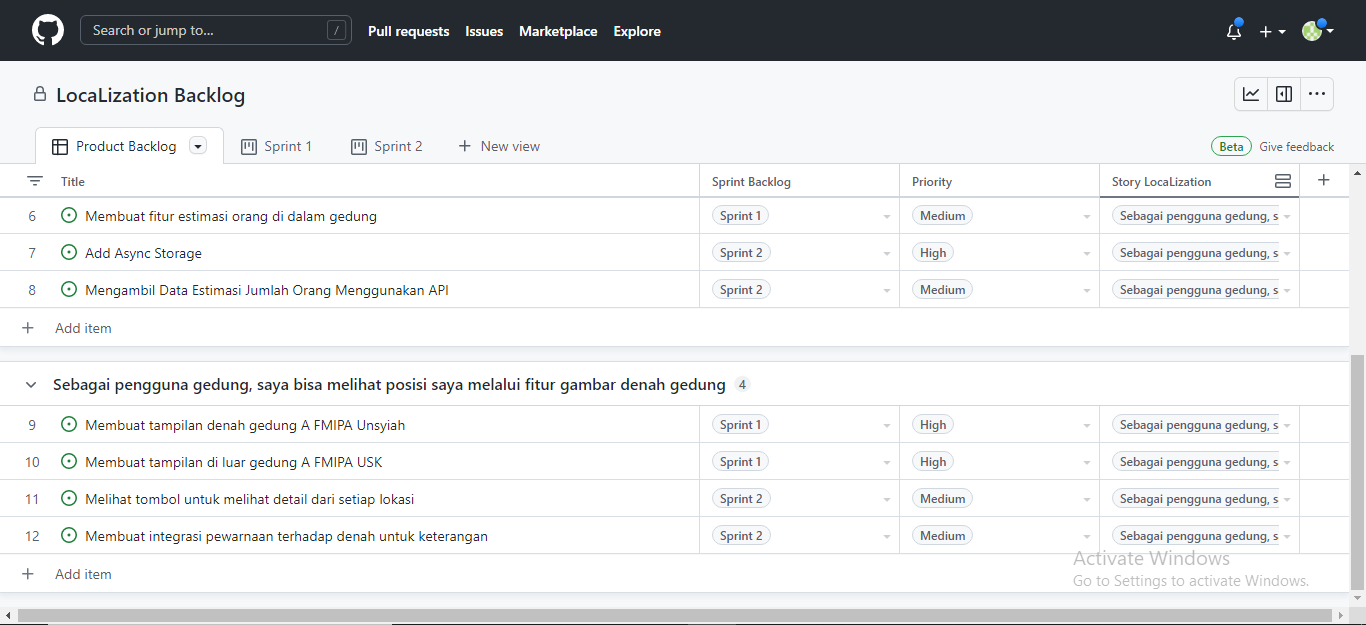
\includegraphics[width=.4\textwidth]{gambar/lampiran/scrum3.PNG}

  \vspace{0.4cm}

  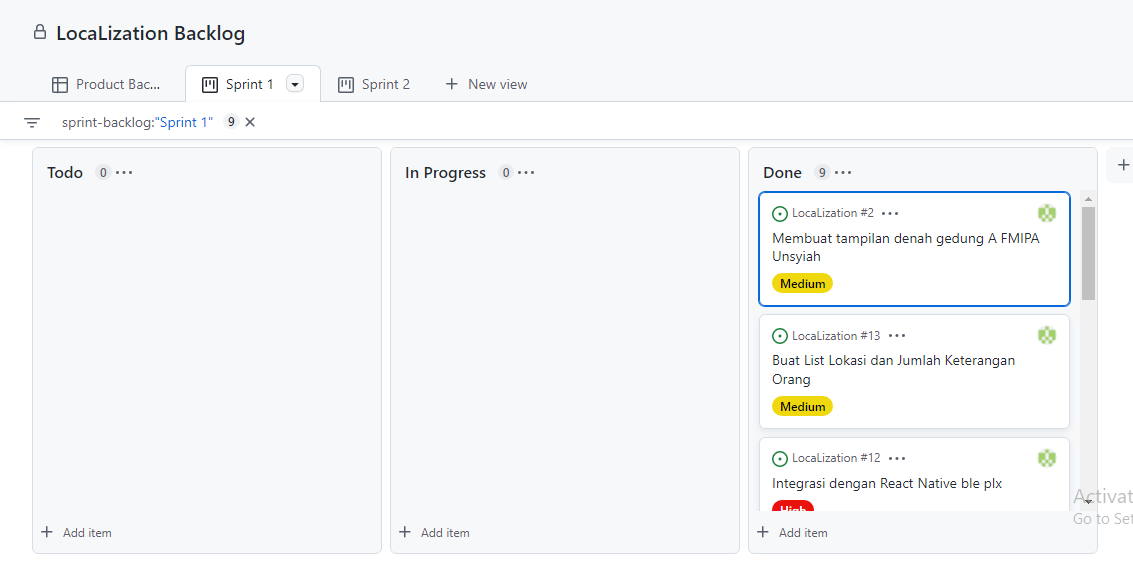
\includegraphics[width=.4\textwidth]{gambar/lampiran/sprint1.PNG}\quad
  \vspace{0.4cm}
  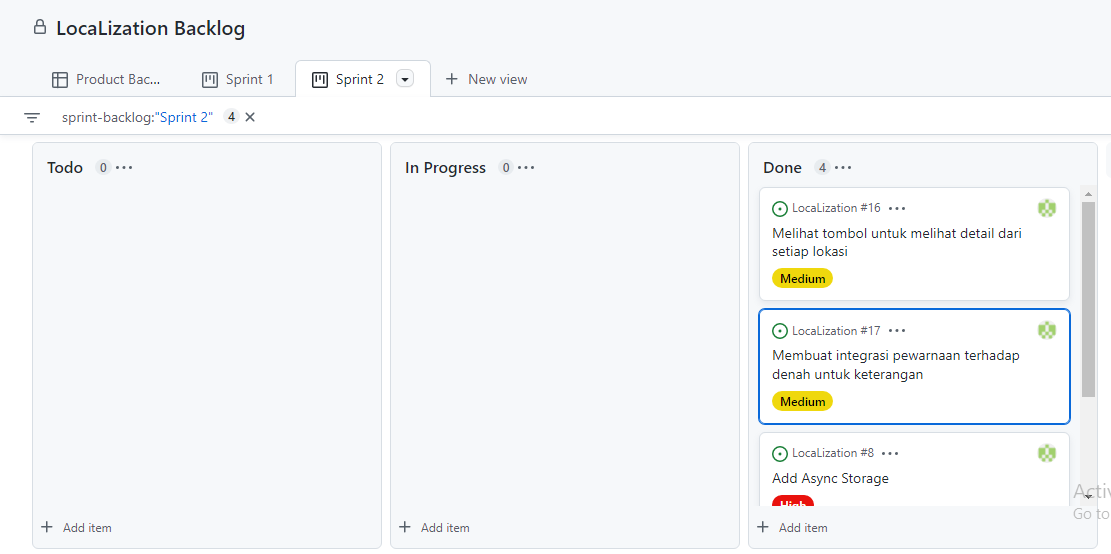
\includegraphics[width=.4\textwidth]{gambar/lampiran/sprint2.PNG}

  \label{sus-mahasiswa}
\end{figure}
%-----------------------------------------------------------------------------%


% Lampiran 4 Laporan Usability

% 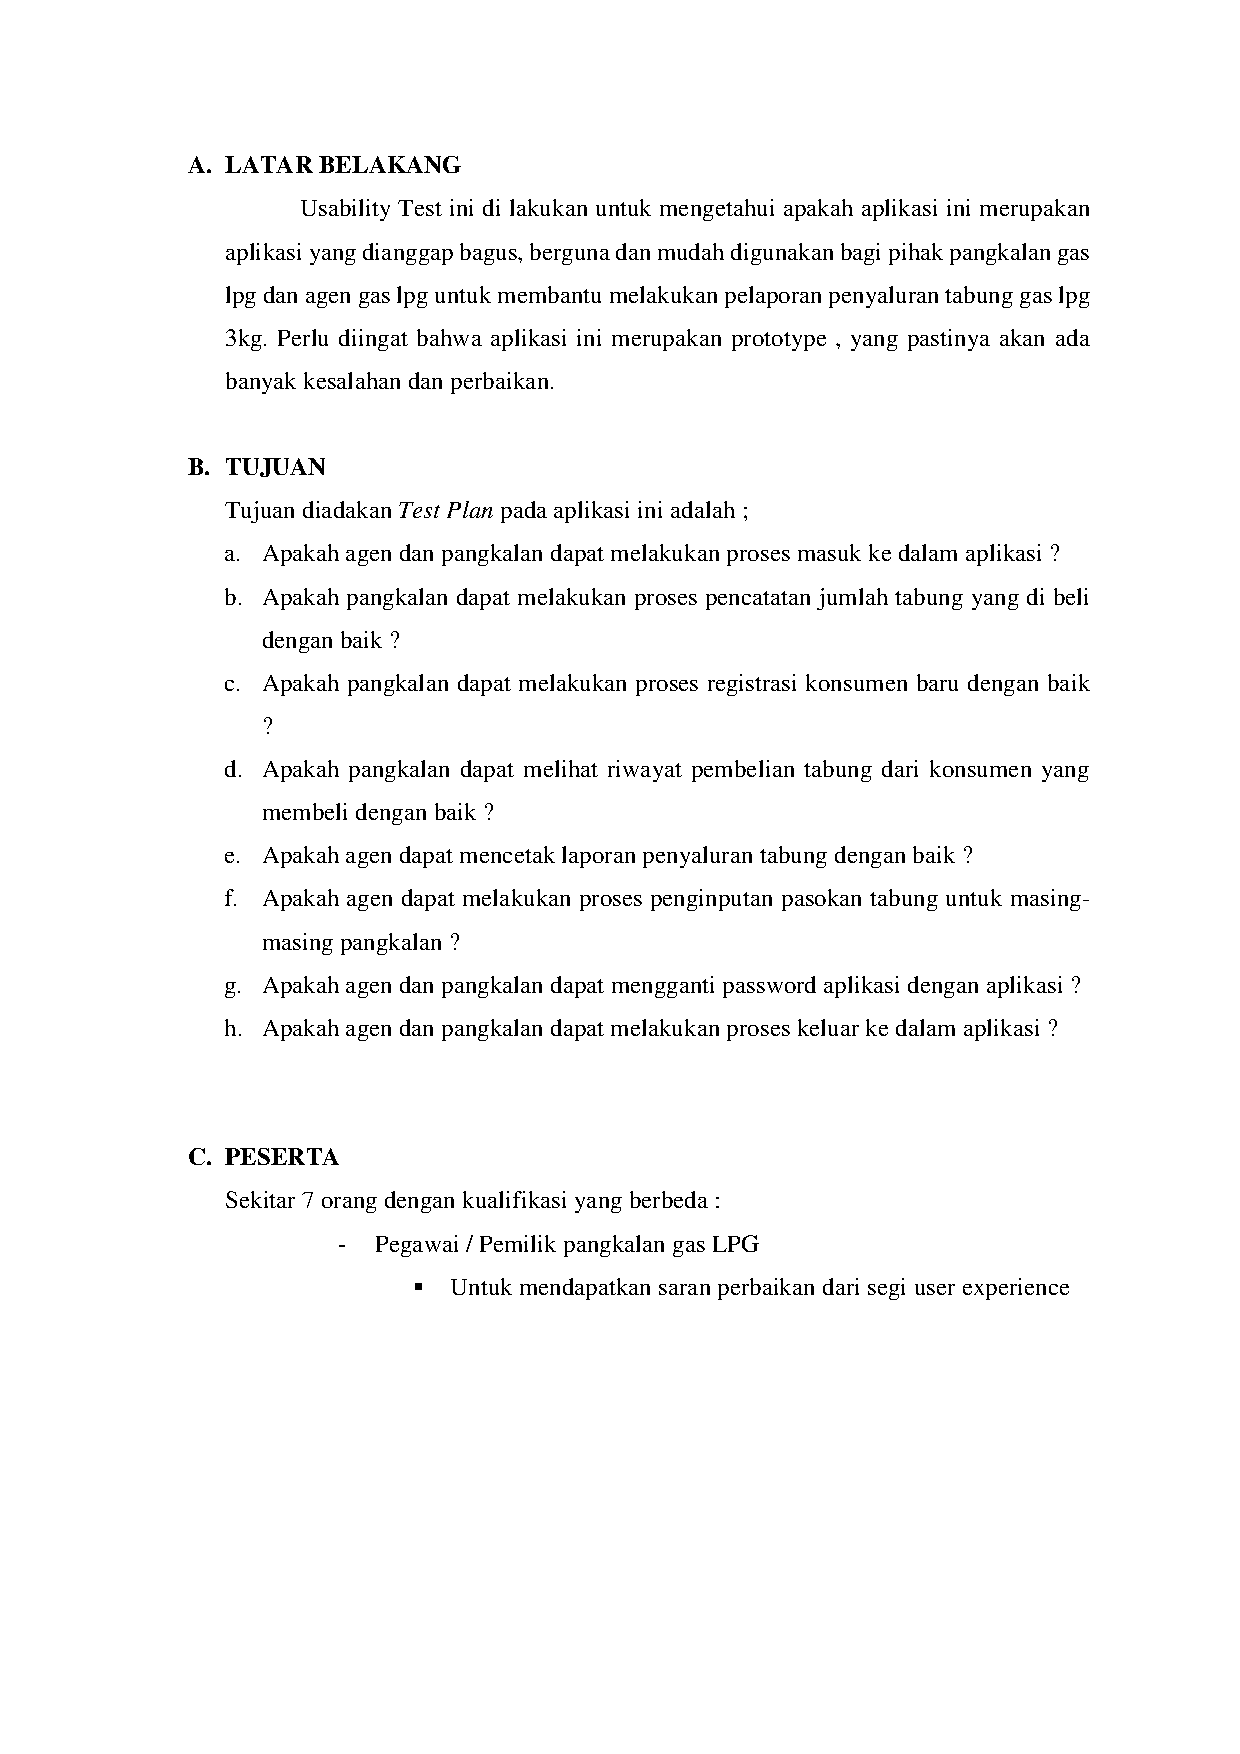
\includepdf[pages=1,scale=.8,pagecommand={
% 	\addcontentsline{toc}{chapter}{LAMPIRAN 4} 
% 	\chapter*{Lampiran 4}
% 	\newappendix{Lampiran 4. Laporan Hasil Pengujian \textit{Usability}}
% },linktodoc=true]{laporan_usability}
% \includepdf[pages=2-,scale=.8,pagecommand={},linktodoc=true]{laporan_usability}
% Lampiran 4 Laporan Usability

% 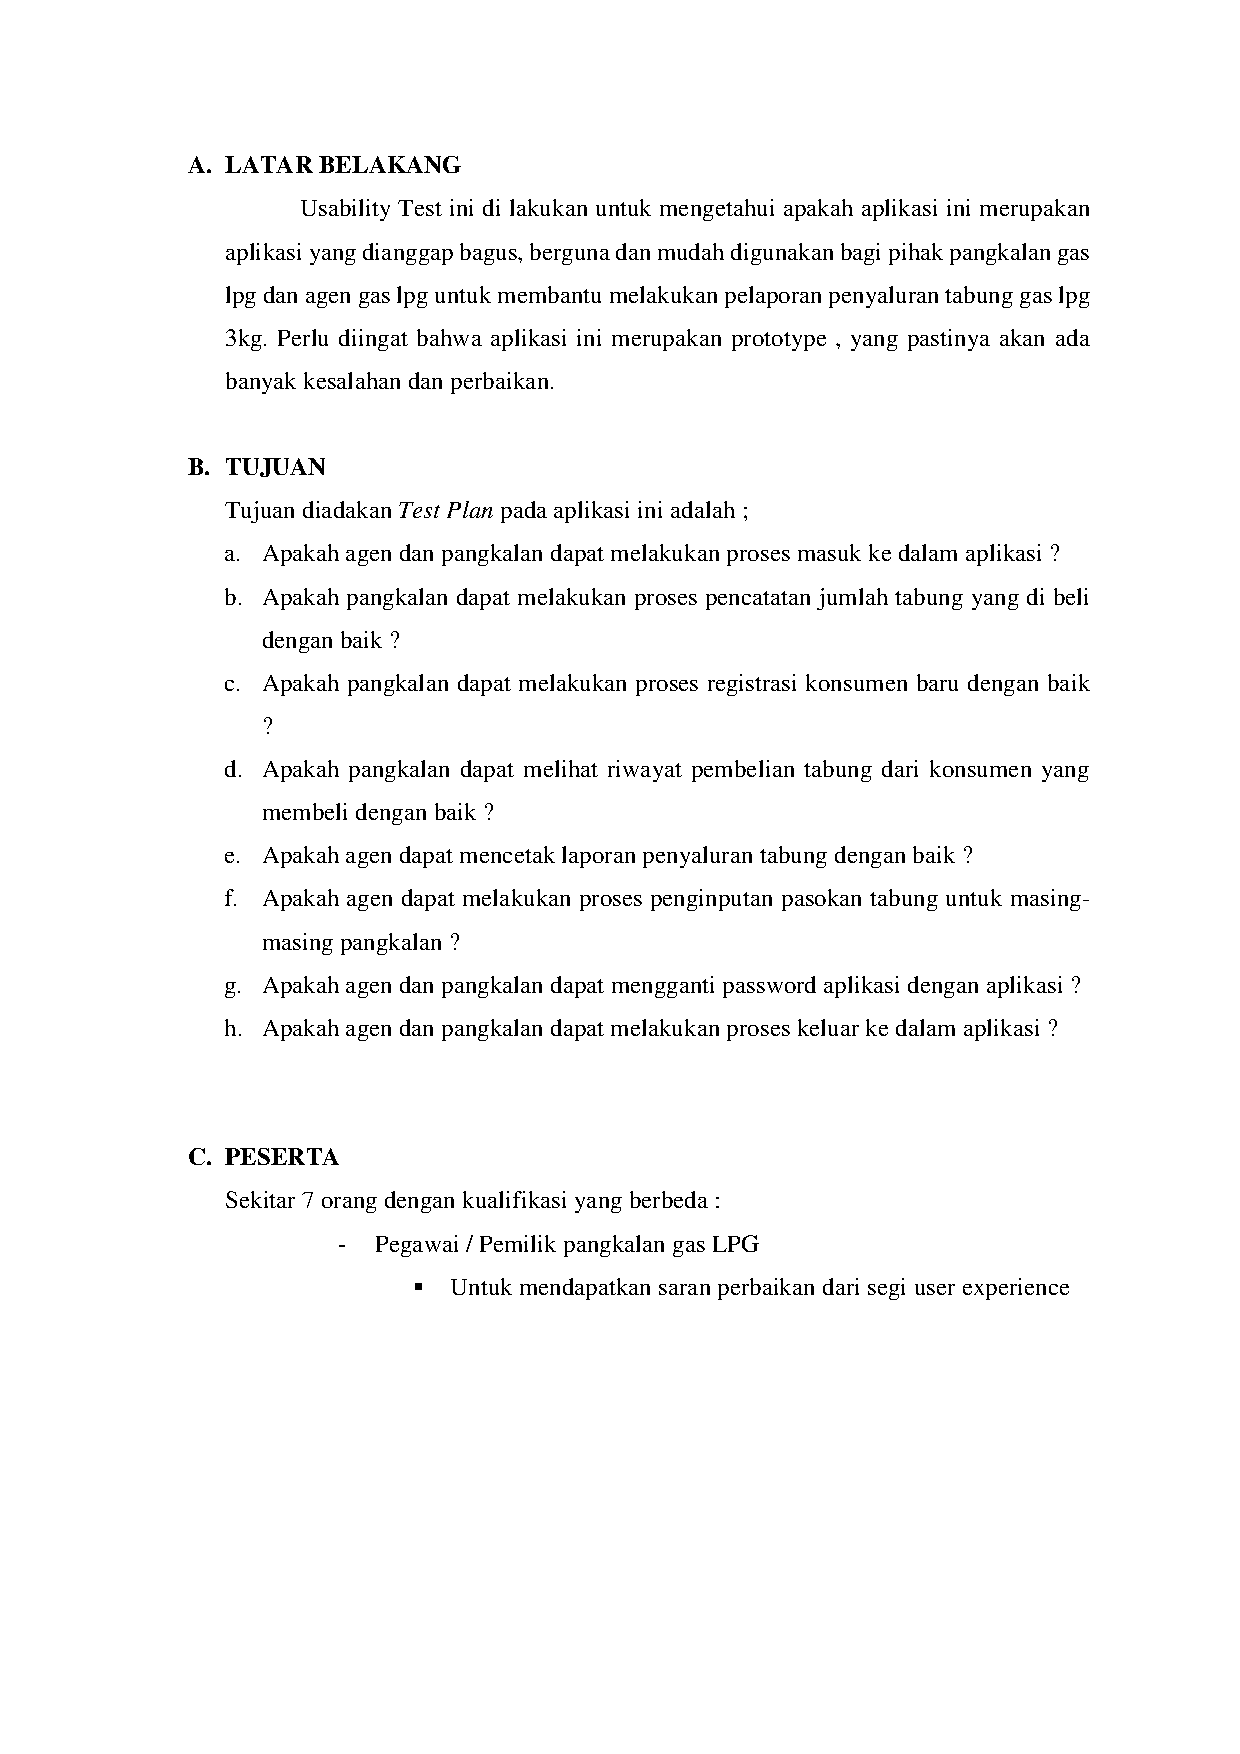
\includepdf[pages=1,scale=.8,pagecommand={
%       \addcontentsline{toc}{chapter}{LAMPIRAN 4}
%       \chapter*{Lampiran 4}
%       \newappendix{Lampiran 4. Laporan Hasil Pengujian \textit{Usability}}
%     },linktodoc=true]{laporan_usability}
% \includepdf[pages=2-,scale=.8,pagecommand={},linktodoc=true]{laporan_usability}